\documentclass[francais, 12pt, fancyChapter, oneside]{these-LUNAM}

\usepackage[utf8]{inputenc}
\usepackage[french,english]{babel}
\usepackage[T1]{fontenc}
%\usepackage{xunicode}
\usepackage{fontspec}
\usepackage{lettrine}

\setmainfont{Crimson}

\usepackage{textcomp}
%\RequirePackage[bookmarks,%
%                colorlinks,%
%                urlcolor=blue,%
%                citecolor=blue,%
%                linkcolor=blue,%
%                hyperfigures,%
%                pagebackref,%
%                pdfcreator=LaTeX,%
%                breaklinks=true,%
%                pdfpagelayout=SinglePage,%
%                bookmarksopen=true,%
%                bookmarksopenlevel=2]{hyperref}

\usepackage{minitoc}
\setcounter{minitocdepth}{2}

\usepackage{url}
\usepackage{algorithm}
\usepackage{paralist}
\usepackage{algorithmicx}
\usepackage{algpseudocode}
\usepackage{amssymb}

\usepackage{times}
\usepackage{fancyhdr}
\usepackage{graphicx}
\usepackage{hyperref}
                                  
\usepackage{booktabs}
\usepackage{multirow}

\usepackage{epstopdf}
\usepackage{epsfig}
\usepackage{subfig}

%% Bibtex
\usepackage[numbers]{natbib}

\usepackage{tikz}
\usetikzlibrary{plotmarks,shapes}
\usetikzlibrary{arrows.meta}
\tikzset{>={Latex[width=3pt,length=4pt]}}

%paralist
\renewcommand*\descriptionlabel[1]{%
\scshape #1}
\renewcommand\paradescriptionlabel[1]{%
\scshape #1}

\usepackage{xspace}
\newcommand{\LSEQ}[0]{\textsc{LSeq}\xspace}
\newcommand{\SCAMP}[0]{\textsc{Scamp}\xspace}
\newcommand{\CYCLON}[0]{\textsc{Cyclon}\xspace}
\newcommand{\SPRAY}[0]{\textsc{Spray}\xspace}
\newcommand{\PEERSIM}[0]{\textsc{PeerSim}\xspace}

%%\titre{Édition collaborative décentralisée}
\titre{Editeur sans frontières}
%%\soustitre{L'exemple de l'édition collaborative}
\title{Editor Without Borders}
%%\subtitle{The collaborative editing use-case}

\author{M.}{Brice}{Nédelec}
\discipline{Informatique et applications}
\institution{UN}
\doctoralschool{Sciences et technologies de l'information, et mathématiques}
\laboratory{Laboratoire d'informatique de Nantes-Atlantique (LINA)}
\date{}

\reviewer{M.}{Prenom}{Nom}{Position}{Location}
\reviewer*{M.}{Prenom}{Nom}{Position}{Location} %% * is not present the d-day

\examiner{M.}{Meow}{Miaw}{Miou}{Miou}
\examiner{M.}{Meow}{Miaw}{Miou}{Miou}
\examiner{M.}{Meow}{Miaw}{Miou}{Miou}
\president{M.}{Miaw}{Miou}{Mew}{Meow}

\guest{Mme}{Miou}{Mi}{aw}{Miou}

\supervisor{M.}{Pascal}{Molli}{Professeur}{Université de Nantes}
\cosupervisor{M.}{Achour}{Mostefaoui}{Professeur}{Université de Nantes}

%%% % %% % %%% %% % %% % %%% % %%% % %% % %% % % %%% 
\newcommand{\TODO}[1]{\textcolor{red}{#1}}
\newcommand{\REF}{\textcolor{purple}{REF}}



\begin{document}

\maketitle

\dominitoc
\tableofcontents
% \listoftables
% \listoffigures

\begin{resume}
  Par défaut, les éditeurs collaboratifs temps réel sur le Web sont
  centralisés. Un serveur du fournisseur de service gère une session
  d'édition. Cela pose des problèmes de confidentialité et de passage à
  l'échelle.  Seulement récemment l'opportunité nous a été offerte d'établir des
  communications d'un navigateur Web à l'autre. Cette possibilité ouvre les
  portes aux applications décentralisées directement accessibles dans les
  navigateurs. Cette thèse comporte trois contributions :
  \begin{inparaenum}[(i)]
  \item Une structure de données répliquée dont la taille des métadonnées passe
    à l'échelle;
  \item Un protocole d'échantillonnage aléatoire de pairs s'ajustant
    automatiquement aux variations de taille du réseau sans connaissances
    globales;
  \item Un éditeur collaboratif temps réel fonctionnant dans les navigateurs Web
    de manière décentralisée utilisant les deux approches ci-dessus.
  \end{inparaenum}
\end{resume}

\begin{motscles}
  Édition collaborative, décentralisé, temps réel, passage à l'échelle,
  structure de donnée répartie pour séquences, échantillonnage aléatoire de
  pairs.
\end{motscles}

\begin{abstract}
  Real-time collaborative editors on the Web are centralized. A service
  provider's server hosts an editing session. It raises privacy and scalability
  issues. Only recently the opportunity to establish browser-to-browser
  communication channels has been enabled. This opens the way to decentralized
  application running directly in web browsers. Contributions of this thesis are
  threefold: 
  \begin{inparaenum}[(i)]
  \item A replicated data structure for sequences using metadata the size of
    which scales;
  \item A random peer sampling protocol that self-adjust its functioning to
    the variations in membership of networks, without global knowledge;
  \item A real-time collaborative editor running in web browsers in a
    decentralized fashion and using the two aforementioned approaches.
  \end{inparaenum}
\end{abstract}

\begin{keywords}
  Collaborative editing, decentralized, real-time, scalable,
  distributed structure for sequences, random peer sampling.
\end{keywords}


  % La récente apparition de la communication de navigateur-à-navigateur a
  % transformé le programme le plus largement répendu en récéptacle à applications
  % web réparties. Chaque navigateur web devient un candidat pour le Fog Computing
  % mélant les avantages du Cloud et du Edge. Cette thèse se concentre sur
  % l'édition collaborative temps réel. Nos contributions comprennent
  % \begin{inparaenum}[(i)]
  % \item un protocole d'échantillonnage aléatoire de pairs qui adapte son
  %   fonctionnement à la taille du réseau sans utiliser de connaissances
  %   globales;
  % \item une structure de données répartie dont la compléxité spatiale est bornée
  %   sous-linéairement comparé à la taille de la séquence.
  % \end{inparaenum}



  % Enabling browser-to-browser communication transformed the most widely spread
  % program into a receptacle for distributed web applications. Each browser
  % becomes an edge-of-the-network candidate for Fog Computing bringing the best
  % of both Cloud and Edge. This thesis focuses on real-time collaborative editing. Our
  % contributions include
  % \begin{inparaenum}[(i)]
  % \item a random peer sampling protocol that adapts its operation to the network
  %   size without any global knowledge. 
  % \item a distributed data structure for sequences that enjoys a sub-linear
  %   upper bound on its space complexity regarding the sequence size.
  % \end{inparaenum}

%%% Local Variables:
%%% mode: latex
%%% TeX-master: "../paper"
%%% End:


%% change spacing in the main document
\setlength{\parskip}{0.5em}



\chapter{Introduction}

\minitoc


Ces dernières années, l'interêt pour les outils collaboratifs n'a eu de cesse
d'augmenter. En particulier, les éditeurs
collaboratifs~\cite{ellis1991groupware} répartis permettent de distribuer la
charge d'écriture d'un document sur les trois dimensions que sont: le temps,
l'espace, et les organisations. Leur utilité ne faisant aucun doute, ces outils
possèdent actuellement de nombreuses limitations. Lorsque l'éditeur est basé sur
un serveur central (par exemple Google Docs~\cite{nichols1995high}), se posent
alors des problèmes liés au point individuel de défaillance, respect de la vie
privée, intelligence économique, censure, et passage à l'échelle. Lorsque
l'éditeur est décentralisé, se posent toujours les problèmes de passage à
l'échelle: nombre d'utilisateurs, concurrence, taille de document etc.

Les applications pair-à-pairs place chaque utilisateur dans le rôle de client et
serveur. Ainsi, non seulement les utilisateurs profitent de l'application
normalement, mais participent au bon fonctionnement de celle-ci. Dès lors, le
serveur central n'est plus nécessaire.

Les éditeurs collaboratifs décentralisés utilisent la réplication
optimiste~\cite{saito2005optimistic} afin de garantir accessibilité et
réactivité des documents partagés. Dans ce type de réplication, chaque
collaborateur possède une réplique locale du document et exécute directement ses
modifications dessus, qui seront partagés dans un second temps à l'ensemble des
participants. Les répliques du documents peuvent diverger temporairement, mais
convergent inéluctablement vers un état identique.

Dans ce manuscrit, nous nous intéressons aux structures de données répliquées
sans résolution de conflits~\cite{shapiro2011comprehensive, shapiro2011conflict}
(CRDTs) appartenant au paradigme de réplication optimiste. Les CRDTs pour
séquences~\cite{ahmed2011evaluating, conway2014language, grishchenko2010deep,
  oster2006data, preguica2009commutative, roh2011replicated, weiss2007wooki,
  wu2010partial, Yu2012stringwise, andre2013supporting, weiss2009logoot}
(structure la plus proche du document) fournissent deux opérations pour modifier
la séquence : l'insertion et la suppression d'un élément. Dans le cadre d'un
document et selon la granularité choisie, ces éléments peuvent être des
caractères, des lignes, des paragraphes etc. Ces deux opérations sont
commutatives, i.e., l'ordre d'intégration de ces opérations n'importe pas. Lors
d'une insertion, le CRDT génère un identificateur unique et immuable qui lui
servira à ordonner la séquence. L'une des familles de CRDTs pour séquence
utilise des identifiants dont la taille est
variable~\cite{preguica2009commutative,
  andre2013supporting,weiss2009logoot}. Dans ces approches, la principale
difficulté consiste à conserver des identifiants de petite taille. La première
contribution présentée dans ce manuscrit concerne une stratégie d'allocation
d'identifiants dont la taille est polylogarithmique par rapport au nombre
d'insertions effectuées sur la séquence~\cite{nedelec2013lseq,
  nedelec2013concurrency}.

Les CRDTs garantissent la cohérence à terme~\cite{bailis2013eventual} sous
l'hypothèse que les opérations arrivent à tous les participants de manière
inéluctable. Les CRDTs nécessitent donc un mécanisme de diffusion des
messages. La dissémination épidémique~\cite{demers1987epidemic,
  eugster2003lightweight, birman1999bimodal} (ou rumeur) est un moyen efficace
d'y parvenir. Chaque pair choisit une liste de pairs et envoie le message. Lors
de la réception d'un tel message, le pair peut choisir d'arrêter la diffusion du
message, ou de le transmettre à son tour à une liste de pairs. Ainsi, selon
toute probabilité, tous les pairs reçoivent le message. Pour obtenir les liste
de pairs, le mécanisme de dissémination peut s'appuyer sur les protocoles
d'échantillonnage aléatoire de pairs~\cite{jelasity2007gossip,
  voulgaris2005cyclon, ganesh2001scamp, tolgyeski2009adaptive,
  eugster2003lightweight}. Ces derniers maintiennent chez chaque pair une liste
de voisins comme vue partielle du réseau entier. Les réseaux générés partagent
de nombreuses similarités avec les graphes aléatoires~\cite{erdos1959random}. En
particulier, ils permettent de maintenir efficacement la connectivité du réseau,
la dissémination d'information, la robustesse aux défaillances etc. La seconde
contribution présentée dans ce manuscrit concerne un protocole d'échantillonnage
aléatoire dont les vues partielles s'adaptent automatiquement à la taille du
réseau, convergeant en temps exponentiel vers une topologie montrant des
similarités avec les graphes aléatoires, et utilisant seulement des interactions
de proche en proche.

Comparé aux approches décentralisées, les éditeurs collaboratifs centralisés ont
l'avantage d'être facile d'accès pour l'utilisateur. Par exemple, Google Docs
est accessible depuis un navigateur web quelconque. Partager un document est
aisé puisqu'il s'agit simplement de donner un lien que le collaborateur puisse
adresser. Toutefois, la récente technologie
WebRTC\footnote{\url{http://www.webrtc.org}} comble ce fossé en permettant la
communication de navigateur à navigateur, et ce, même avec des configurations
réseau complexes impliquant firewall, proxy, ou NAT (Network Address
Translation). En particulier, WebRTC étend le champs d'utilisateurs aux
dispositifs limités en ressource comme les smartphones, tablettes etc. Dans la
troisième partie de ce manuscrit est présenté CRATE (CollaboRATive Editor), un
éditeur collaboratif décentralisé et réparti dont le coeur est composé de LSEQ
(la stratégie d'allocation présenté en première partie) et Spray (le protocole
d'échantillonnage présenté en seconde partie) et accessible depuis un navigateur
web.



\section{Objectifs et contributions}

%%% Local Variables:
%%% mode: latex
%%% TeX-master: "../../paper"
%%% End:


\section{Organisation du manuscrit}

%%% Local Variables:
%%% mode: latex
%%% TeX-master: "../../paper"
%%% End:


\part{Réplication de données}
\chapter{Schémas de réplication}

\lettrine{L}a maintenance de répliques sur des machines distantes les unes des
autres est un problème ancien. Dès 1976, les bases de données répliquées font
leur apparition afin de résoudre les problèmes de défaillances, i.e., le serveur
possédant les données étant inaccessible, le client peut contacter serveur
alternatif connu pour posséder les mêmes données afin de satisfaire sa requête.

Hélas, avec la réplication, la synchronisation de répliques devient le coeur du
problème. Puisque la communication entre serveurs n'est pas instantanée, les
modifications effectuées sur les données prennent du temps à parvenir aux
répliques. Cela implique des problèmes de
\begin{inparaenum}[(i)]
\item fraîcheur de données -- \emph{est-ce que la donnée que j'obtiens est la
    plus à jour?} -- et de
\item modifications concurrentes -- \emph{avec des modifications effectuées sur
    une même données, au même moment, par deux serveurs distants dont les
    résultats sont différents. Dois-je conserver les deux modifications, ou
    dois-je en privilégier une, ou dois-je employer une autre stratégie?}
\end{inparaenum}

D'après le bien connu théorème CAP~\cite{gilbert2002brewer} (\emph{Consistency,
  Availability, Partition tolerence}), il est impossible de \TODO{passer à
  l'échelle} tout en garantissant à la fois \TODO{
\begin{itemize}
\item la cohérence : un contrat entre le développeur et la structure qui
  spécifie comment cette dernière se comporte suivant les opérations effectuées
  et leur ordonancement. Les contraintes imposées à la structure peuvent être
  plus ou moins importantes selon les besoins.
\item la disponibilité : le ratio entre le temps effectif durant lequel
  l'utilisateur accède à un service et le temps durant lequel il souhaite y
  accèder. Dans le meilleur cas, le service est toujours disponible. \TODO{La
    plupart des services \emph{Cloud} proposent de 99 à 100\% (exclus) de
    disponibilité.}
\item la tolérance aux pannes : \TODO{les défaillances n'entrainent pas de defauts
  dans les propriétés susmentionnées}.
\end{itemize}
}

Face à ce constat, deux familles de réplication existent proposant différents
compromis. La section~\ref{repl:sec:pessimistic} décrit succintement les
approches dîtes pessimistes dont le critère de cohérence est fort mais ne
pouvant s'appliquer à grande échelle. À l'opposé, la
section~\ref{repl:sec:optimistic} décrit la réplication optimiste dont le
critère de cohérence est plus faible mais pouvant atteindre une plus grande
échelle.

\section{Réplication pessimiste}
\label{repl:sec:pessimistic}

L'objectif de la réplication pessimiste est simple. Il consiste à donner
l'illusion qu'indépendemment du nombre de répliques, il existe une donnée
unique.

\section{Réplication optimiste}

En 1987, Demers et al. décrivent une base de données répliquée sur plusieurs
centaines de machines pouvant communiquer entre elles au travers de materiels
aux capacités hétérogènes~\cite{demers1987epidemic}.

\section{Conclusion}

Depuis les premières base de données répliqués, les dimensions ont
considérablement augmentées mais les problématiques restent identiques. Les
réseaux \TODO{pair-à-pair} transforment chaque \TODO{client} en
client-serveur. Chaque utilisateur final possède alors une réplique de la donnée
partagée. Dans ce contexte, il est inenvisageable d'en appeler à la réplication
pessimiste. 




\chapter{Structure de données sans résolution de conflits}
\section{Transformés opérationnels}
\section{Compteur}
\section{Ensembles}
\section{Composition}
\section{Conclusion}

\chapter{Séquences répliquées}
\section{Introduction}
\section{Pierre tombales}
\subsection{Woot}
\section{Identifiant de taille variable}
\subsection{Logoot}
\subsection{Treedoc}

%%\part{Transmission d'informations}
%%\chapter{Appartenance réseau}
%%\chapter{Diffusion}
%%\part{CRATE : un éditeur collaboratif décentralisé}
%%\chapter{LSEQ}
%%\chapter{SPRAY}

%%\chapter{Structure de données répliquée : la séquence}
%%\minitoc
%%
\section{Introduction}

\lettrine{L}a réplication optimiste permet de garantir accessibilité et
réactivité en copiant les données partagées directement chez
l'utilisateur. Ainsi, chaque utilisateur applique ses opérations sur sa copie et
les communique aux autres détenteurs de copies afin qu'ils ajustent l'état de
leur propre copie.

Dans ce chapitre, nous nous intéressons aux séquences répliquées \TODO{(Eventual
  consistency, decentralized?)} permettant, par exemple, de représenter des
documents. Les plus anciennes approches se nomment les \emph{transformés
  opérationelles}. Comme leur nom l'indique, celles-ci modifient les opérations
réçues par rapport aux opérations effectuées en concurrence à
celles-ci. Malheureusement ce procédé peut s'avérer coûteux aussi bien en temps
qu'en espace.  Afin de réduire ce coût, des structures de données répliquées
furent proposées. Elles s'affranchissent des vérifications de concurrence grâce
à des opérations dont les résultats sont commutatifs entre eux. Ainsi, quel que
soit l'ordre d'intégration des opérations, les répliques convergent vers un
état équivalent.

Nous distinguons deux familles de structure. La première utilise des
\emph{pierres tombales} afin d'indiquer qu'un élément de la séquence a été
supprimé. Elles sont nécéssaires car la position de l'élément, bien que
supprimé, reste importante pour la suite de l'exécution. Malheureusement,
supprimer ces pierres tombales requière l'utilisation d'un ramasse-miète réparti
dont le coût est encore plus prohibitif que ces premières. La seconde famille
utilise des identifiants dont la taille varie à la génération. Hélas, cette
taille dépend des positions où les éléments sont insérés. \TODO{more}

La section~\ref{lseq:sec:stateoftheart} de ce chapitre présente l'état de l'art
des approches appartenant à la réplication optimiste de séquences. La
section~\ref{lseq:sec:proposal} détaille \LSEQ, une stratégie d'allocation dont
les identifiants jouissent d'une complexité spatiale sous-linéaire comparée à la
taille de la séquence. La section~\ref{lseq:sec:experiments} valide notre
approche au travers d'expérimentations \TODO{large échelle}. Enfin, nous
\TODO{concluons et discutons} en section~\ref{lseq:sec:conclusion}.

%%% Local Variables:
%%% mode: latex
%%% TeX-master: "../../paper"
%%% End:

%%
\section{État de l'art}

\label{lseq:sec:stateoftheart}

\subsection{Réplication optimiste}

La réplication optimiste~\cite{demers1987epidemic, saito2005optimistic} est un
paradigme de réplication qui consiste à copier la donnée partagée chez chaque
utilisateur. De cette façon, ces derniers peuvent directement modifier les
copies, et ce, même en cas de déconnexions.  Ainsi, les données sont toujours
disponibles et réactives aux changements effectués. Dans un second temps, les
modifications sont disséminées aux autres possesseurs de cette donnée partagée
où elles sont appliquées à la copie locale.

D'après le théorème CAP~\cite{gilbert2002brewer} (\emph{Consistency,
  Availability, Partition tolerence}), il est impossible de passer à l'échelle
tout en garantissant à la fois
\begin{itemize}
\item la cohérence : un contrat entre le développeur et la structure qui
  spécifie comment cette dernière se comporte suivant les opérations effectuées
  et leur ordonancement. Les contraintes imposées à la structure peuvent être
  plus ou moins importantes selon les besoins.
\item la disponibilité : le ratio entre le temps effectif durant lequel
  l'utilisateur accède à un service et le temps durant lequel il souhaite y
  accèder. Dans le meilleur cas, le service est toujours disponible. \TODO{La
    plupart des services \emph{Cloud} proposent de 99 à 100\% (exclus) de
    disponibilité.}
\item la tolérance aux pannes : \TODO{les défaillances n'entrainent pas de defauts
  dans les propriétés susmentionnées}.
\end{itemize}

La réplication optimiste choisit de sacrifier sur le critère de cohérence au
profit de la disponibilité et de la tolérance aux pannes: lorsque les mêmes
changements ont été reçus et appliqués par tous les participants, les copies
convergent vers un état équivalent. Il s'agit du critère de cohérence
correspondant à la cohérence à terme forte~\cite{shapiro2011conflict} (ou
cohérence inéluctable forte). Bien qu'il soit possible de garantir d'avantages
de propriétés, notamment sur l'ordonnancement des modifications, nous nous
intéresserons principalement à ce critère de cohérence.

\begin{figure}
  \centering
  
\begin{tikzpicture}[scale=1.2]

  \newcommand\X{30pt};
  \newcommand\Y{30pt};
  
  \draw[->](0pt,   0pt)--(10*\X,   0pt);
  \draw[->](0pt, -1*\Y)--(10*\X, -1*\Y);
  \draw[->](0pt, -2*\Y)--(10*\X, -2*\Y);
  
  \draw[fill=black](0pt, 0pt) node[anchor=east]{copie 1 }circle(2pt);
  \draw[fill=black](0pt, -1*\Y) node[anchor=east]{copie 2 }circle(2pt);
  \draw[fill=black](0pt, -2*\Y) node[anchor=east]{copie 3 }circle(2pt);

  \draw(\X,2pt)--node[anchor=south]{[ ]}( \X,   -2pt);
  \draw(\X,2 -1*\Y)--node[anchor=south]{[ ]}(\X,-2 -1*\Y);
  \draw(\X,2 -2*\Y)--node[anchor=south]{[ ]}(\X,-2 -2*\Y);

  \draw(2* \X,2pt)--node[anchor=south]{[QWE]}(2* \X,   -2pt);
%  \draw(2* \X,2 -1*\Y)--node[anchor=south]{[ ]}(2* \X,-2 -1*\Y);
%  \draw(2* \X,2 -2*\Y)--node[anchor=south]{[ ]}(2* \X,-2 -2*\Y);

  \draw[->, dashed] (2*\X, 0pt) -- (8*\X, -1*\Y);
  \draw[->, dashed] (2*\X, 0pt) -- (3*\X, -2*\Y);

  \draw(4*\X, 2 -0*\Y)--node[anchor=south]{[QWE]}(4*\X,-2 -0*\Y);
  \draw(4*\X, 2 -1*\Y)--node[anchor=south]{[ ]}(4*\X,-2 -1*\Y);
  \draw(4*\X, 2 -2*\Y)--node[anchor=south]{[QWE]}(4*\X,-2 -2*\Y);


  \draw(6*\X, 2 -2*\Y)--node[anchor=north]{[QWERTY]}(6*\X,-2 -2*\Y);


  \draw[->, dashed] (6*\X, -2*\Y)--(7*\X, -0*\Y);
  \draw[->, dashed] (6*\X, -2*\Y)--(7*\X, -1*\Y);

  \draw(9*\X, 2 -0*\Y)--node[anchor=south]{[QWERTY]}(9*\X,-2 -0*\Y);
  \draw(9*\X, 2 -1*\Y)--node[anchor=south]{[QWERTY]}(9*\X,-2 -1*\Y);
  \draw(9*\X, 2 -2*\Y)--node[anchor=south]{[QWERTY]}(9*\X,-2 -2*\Y);


%%  \draw[fill=white, very thick]
%%  (0*\X, 0*\Y) node{$p_1$} +(-5pt,-5pt) rectangle +(5pt,5pt);
%%  \draw[->](-5+\X, 5+2*\Y)to[out=120,in=30](0pt,5+2*\Y); %% 6 -> 7
\end{tikzpicture}
  \caption{\label{lseq:fig:optimisticexample}Exemple d'exécution d'un protocole
    de réplication optimiste. Il existe trois copies d'une séquence initialement
    vide. La première copie insère 'QWE' et en dissémine l'information. La
    troisième copie reçoit l'opération et l'applique localement. Cette copie
    insère 'RTY' à la suite de 'QWE' afin d'obtenir 'QWERTY' et envoie
    l'information aux deux autres copies. Quel que soit l'ordre de réception, le
    protocole garanti que les copies convergent vers un état identique, ici, la
    séquence 'QWERTY'.}
\end{figure}

La figure~\ref{lseq:fig:optimisticexample} présente un cas de séquence
répliquée. Quel que soit l'ordre de reception des opérations et leur nature, les
copies convergent toute vers un état identique : la séquence QWERTY.

Les approches de réplication optimiste pour séquences se divisent en deux
catégories. Les premiers utilisent les transformés
opérationnels~\cite{sun1998operational, sun2009contextbased} qui, lors de la
réception d'une modification, en change les paramètres égards des opérations
concurrentes. Les seconds utilisent un type de données
commutatif~\cite{shapiro2011comprehensive, shapiro2011conflict} où l'envoie
n'est pas l'opération mais son résultat qui, après réception, est intégré à la
structure.

\subsection{Transformés opérationnels}

Les approches à transformés opérationnels~\cite{sun1998operational,
  sun2009contextbased} (OT) sont les plus anciennes et s'appliquent à un large
champs d'applications tels que l'édition de texte, l'édition d'images etc. Dans
le cadre de l'édition de texte, en plus des usuelles opérations d'insertion et
de suppression, OT founit des opérations ciblant les chaînes de caractères
telles que le déplacement, le couper -- coller, etc. Toutefois, l'analyse de
correction nécessite d'examiner chaque paire d'opérations ainsi que leurs
paramètres. En conséquence, lors de l'écriture du papier
\cite{imine2003proving}, peu d'approches étaient réellement correctes. De plus,
cette classe d'approches peut être divisé en deux sous-classes: les approches
centralisées et les approches décentralisées. Les premières réarrangent les
opérations sur un serveur central~\cite{nichols1995high} afin de faciliter la
convergence. Toutefois, la topologie elle-même implique un point individuel de
défaillance, des problèmes de confidentialité, des problèmes d'intelligence
économique, des problèmes de censure, et enfin, de passage à l'échelle. Les
approches décentralisées~\cite{sun2009contextbased}, quant à elle, nécessitent
un vecteur de version afin d'identifier les contextes de génération des
opérations reçues. Elles transforment les arguments de l'opération reçue par
rapport aux opérations concurrentes dans le but d'exécuter de manière cohérente
l'opération sans avoir à défaire et réexecuter ces opérations. De ce fait, bien
que l'exécution locale d'une opération soit très efficace, l'exécution des
opérations reçues est très coûteuse en cas de concurrence. Ainsi, confiné aux
environnements maîtrisés, OT reste efficace~\cite{mehdi2014merging}.

\begin{figure}
  \centering
  
\begin{tikzpicture}[scale=1.2]

  \newcommand\X{30pt};
  \newcommand\Y{30pt};
  
  \draw[->](0pt,   0pt)--(10*\X,   0pt);
  \draw[->](0pt, -1*\Y)--(10*\X, -1*\Y);
  \draw[->](0pt, -2*\Y)--(10*\X, -2*\Y);
  
  \draw[fill=black](0pt, 0pt) node[anchor=east]{copie 1 }circle(2pt);
  \draw[fill=black](0pt, -1*\Y) node[anchor=east]{copie 2 }circle(2pt);
  \draw[fill=black](0pt, -2*\Y) node[anchor=east]{copie 3 }circle(2pt);

  \draw(\X,2pt)--node[anchor=south]{[RTY]}( \X,   -2pt);
  \draw(\X,2 -1*\Y)--node[anchor=south]{[RTY]}(\X,-2 -1*\Y);
  \draw(\X,2 -2*\Y)--node[anchor=south]{[RTY]}(\X,-2 -2*\Y);
  \small
  \draw(3* \X,2pt)--node[anchor=north]{$insert(QWE,\,0)$}(3 * \X,   -2pt);
  \draw(3* \X,2 -2*\Y)--node[anchor=north]{$delete(0,\,3)$}(3 * \X,-2 -2*\Y);
  \normalsize

  \draw(3* \X,2pt)--node[anchor=south]{[QWERTY]}(3 * \X,   -2pt);
%  \draw(2* \X,2 -1*\Y)--node[anchor=south]{[ ]}(2* \X,-2 -1*\Y)
  \draw(3* \X,2 -2*\Y)--node[anchor=south]{[ ]}( 3 * \X,-2 -2*\Y);

  \draw[->, dashed] (3*\X, 0pt) -- (7*\X, -1*\Y);
  \draw[->, dashed] (3*\X, 0pt) -- (7*\X, -2*\Y);

  \small
  \draw[->, dashed] (5*\X, -2*\Y) -- (7*\X,  0*\Y)
  node[anchor=south]{$delete(3,\,3)$};
  \normalsize
  \draw[->, dashed] (5*\X, -2*\Y) -- (7*\X, -1*\Y);

  \draw(9*\X, 2 -0*\Y)--node[anchor=south]{[QWE]}(9*\X,-2 -0*\Y);
  \draw(9*\X, 2 -1*\Y)--node[anchor=south]{[QWE]}(9*\X,-2 -1*\Y);
  \draw(9*\X, 2 -2*\Y)--node[anchor=south]{[QWE]}(9*\X,-2 -2*\Y);


%%  \draw(9*\X, 2 -0*\Y)--node[anchor=south]{[QWERTY]}(9*\X,-2 -0*\Y);
%%  \draw(9*\X, 2 -1*\Y)--node[anchor=south]{[QWERTY]}(9*\X,-2 -1*\Y);
%%  \draw(9*\X, 2 -2*\Y)--node[anchor=south]{[QWERTY]}(9*\X,-2 -2*\Y);


%%  \draw[fill=white, very thick]
%%  (0*\X, 0*\Y) node{$p_1$} +(-5pt,-5pt) rectangle +(5pt,5pt);
%%  \draw[->](-5+\X, 5+2*\Y)to[out=120,in=30](0pt,5+2*\Y); %% 6 -> 7
\end{tikzpicture}
  \caption{\label{lseq:fig:otexample}Exemple de transformé opérationnel
    garantissant la convergence lors d'opérations concurrentes. L'opération de
    suppression des 3 premiers caractères sur la copie 3 (RTY) est transformée
    afin de supprimer les 3 caractères à l'index 3 sur les autres copies.}
\end{figure}

La figure~\ref{lseq:fig:otexample} illustre le principe de fonctionnement des
approches basées sur les transformés opérationnels. Dans ce scenario, les copies
sont toutes initialisées avec la séquence RTY. Ensuite, tandis que la copie 1
insère les 3 caractères QWE en tête de la séquence pour obtenir QWERTY, la copie
3 supprime ses trois caractères pour obtenir la séquence vide. Avant la
dissémination de ces opérations, les copies ne sont pas identiques. Les copies
1, 2, et 3 ont respectivement les séquences [QWERTY], [RTY], []. Lorsque la
copie 1 réçoit l'opération de suppression, elle détecte que cette dernière est
en concurrence avec des opérations déjà intégrées, en l'occurence,
$insert(QWE,\,0)$. Son objectif est alors de déterminer l'impact que cette
opération concurrente a eu sur l'opération réçue afin d'en adapter les
arguments. Ici, l'insertion a décalé la séquence RTY de 3 positions vers la
droite. Par conséquent, La suppression, de part sa position, est elle aussi
décalée de 3 positions vers la droite. La résultat de la transformation est
$delete(3,\,3)$.  La copie 3, lorsqu'elle réçoit l'opération d'insertion,
detecte elle aussi que cette dernière est concurrente. Toutefois, la
transformation est sans effet sur ses arguments. La copie 2, selon l'ordre de
réception, se comporte comme la copie 1 ou la copie 3. À terme, les trois copies
convergent vers une séquence identique QWE.

\subsection{Structures de données sans résolution de conflits}

Plus récemment, les approches à base de \emph{structures de données répliqués
  sans résolution de conflits}~\cite{shapiro2011comprehensive,
  shapiro2011conflict} (CRDTs) commencèrent à émerger. Ces types de structure
abstraits possèdent la particularité de fournir des opérations dont les
résultats sont commutatifs entre eux.  En d'autres termes, le résultat de
l'exécution locale de chaque opération est envoyé aux possesseur de réplique et
peut directement être intégré à cette dernière.  L'ordre d'intégration des
opérations n'importe pas. Cela permet de grandement alléger, voir supprimer, le
coût d'ordonnancement des opérations. Ce genre de structure existe pour les
compteurs, les ensembles, les graphes orientés acycliques (DAG) etc.

Une importante différence entre les approches basées sur OT et les approches
basées sur les CRDTs réside dans la répartition des coûts algorithmiques entre
exécution locale et intégration distante. En effet, OT propose des opérations
sans coût additionnel localement, mais dont le coût est élevé à l'intégration.
En revanche, les approches CRDTs répartissent les coûts entre la partie locale
et l'intégration.  L'impact étant d'autant plus important qu'une opération local
génère autant d'intégrations que de répliques.

\TODO{Tandis que les CRDTs améliorent de manière significative la complexité
temporelle des opérations comparé aux approches OT décentralisées, ils
dissimulent leur complexité dans l'occupation mémoire. En effet, afin d'assurer
la convergence des répliques, une opération d'insertion alloue un identifiant
unique.}

\subsubsection{Le compteur}

L'exemple du CRDT pour compteur permet d'introduire l'idée sur laquelle ils se
fondent. \TODO{Par la suite, on note
  $op_a \times op_b \times \ldots \times op_n$ une séquence d'opérations.}


Un compteur est simplement un entier proposant aux utilisateurs de l'incrémenter
de 1. Si 3 utilisateurs incrémentent chacun leur compteur, les répliques du
compteur convergeront inéluctablement vers la valeur 3. Dans ce cas, il est
clair que l'ordre d'intégration des opérations importe peu :
\begin{equation}
  Inc_a \times Inc_b = Inc_b \times Inc_a \, \, \, (commutative)
\end{equation}

Ainsi, l'origine de l'incrémentation ($a$ ou $b$) n'influence pas le résultat.
Toutefois, il est nécessaire de s'assurer qu'aucune opération n'est appliquée
plusieurs fois. Ainsi, chaque opération est identifiée de manière unique de telle
sorte que :
\begin{equation}
  Inc_a \times Inc_a = Inc_a \, \, \, (idempotence)
\end{equation}

Les identifiants accompagnant chaque opération constituent le surcoût des
approches CRDTs. D'une manière ou d'une autre, il est nécéssaire de les
enregistrer afin de garantir que la structure progresse continuellement. Par
exemple, l'implémentation de ce compteur peut se faire sous la forme d'un
ensemble répertoriant tous les identifiants. Sa valeur est le cardinal de cet
ensemble.

Considérons maintenant que le compteur propose une opération supplémentaire, à
savoir la décrémentation de 1. Une implémentation naïve consisterait à supprimer
un élément de l'ensemble aléatoirement. Toutefois, si deux utilisateurs
suppriment en concurrence (autrement dit en même temps) le même élément, alors
le compteur ne serat globalement décrémenté que de 1. Une autre implémentation
plus coûteuse consiste à associer un identifiant unique par décrémentation et
les placer dans un ensemble différent. La valeur du compteur est alors égale au
cardinal des incrémentations moins le cardinal des décrémentations. Cela
correspond aux approches à pierre tombales décritent en
section~\ref{lseq:subsubsec:tombstones}. La structure grandit linéairement par
rapport aux opérations effectuées sur celle-ci.  

Une autre implémentation de ce compteur consiste à sauvegarder un vecteur d'état
recensant le nombre d'incrémentations et de décrémentations effectuées par
chaque utilisateur. Ainsi, la structure grandit linéairement par rapport au
nombre d'utilisateurs ayant jamais effectué une opération sur le compteur
réparti (\TODO{max(received value)}). Cette optimisation est possible car aucune
des opérations ne dépend d'une autre pour être menée à bien. La
section~\ref{lseq:subsubsec:variable} présente un autre type d'optimisation lié
à la séquence.

Le cas du CRDTs pour compteur met en lumière qu'il existe plusieurs
implémentations proposant des compromis différent.  Toutefois, quelle que soit
la structure, elles coûtent beaucoup plus cher que leurs homologues
non-répartis. Il est nécéssaire d'analyser avec prudence les besoins de
l'application afin de choisir au mieux son compromis entre temps, espace, et
communication. La suite de ce chapitre s'attache à décrire les approches CRDTs
dédiées aux séquences.

\subsubsection{Pierres tombales}
\label{lseq:subsubsec:tombstones}

Les approches utilisant des pierres tombales~\cite{ahmed2011evaluating,
  conway2014language, grishchenko2010deep, oster2006data,
  preguica2009commutative, roh2011replicated, weiss2007wooki, wu2010partial,
  yu2012stringwise} se caractérisent par la manière dont les suppressions sont
traitées. En effet, lors de l'opération $delete$, ces approches marquent
simplement les éléments supprimés afin de les cacher à l'utilisateur. Bien que
supprimées, ces pierres tombales existent toujours dans la structure
représentant la séquence et continuent d'impacter sur les performances.

Le premier représentant historique appartenant à cette famille de CRDT se nomme
WOOT~\cite{oster2006data}. Lors de l'insertion d'un élément dans la séquence,
l'identifiant généré référence simplement les identifiants voisins à
l'insertion. Par exemple, considérons la chaîne QWETY dont les identifiants
respectifs à chaque caractère sont $i_Q$,$i_W$,\ldots,$i_Y$. Lors de l'insertion
du caractère R entre les caractères E et T, l'identifiant généré est composé de
$i_E$ et $i_T$ respectivement référencés comme étant la borne inférieur et
supérieur du nouvel élément. Lors de l'intégration, un diagramme de Hasse permet
de retrouver l'ordre des éléments de la séquence, même en présence d'opérations
concurrentes. 

\begin{figure}
  \centering
  
\begin{tikzpicture}[scale=1.2]

\newcommand\X{ 40pt}
\newcommand\Y{ 30pt}

\draw[fill=white](0 * \X, 0 * \Y) node{$\vdash$}+(-5pt,-5pt)rectangle+(5pt,5pt);
\draw[fill=white](7 * \X, 0 * \Y) node{$\dashv$}+(-5pt,-5pt)rectangle+(5pt,5pt);

\draw[fill=white](1 * \X, 1 * \Y) node{\textbf{Q}}+(-5pt,-5pt)rectangle+(5pt,5pt);
\draw[fill=white](2 * \X, 1 * \Y) node{\textbf{W}}+(-5pt,-5pt)rectangle+(5pt,5pt);

\draw[fill=white](1 * \X, 0 * \Y) node{\textbf{A}}+(-5pt,-5pt)rectangle+(5pt,5pt);
\draw[fill=white](2 * \X, 0 * \Y) node{\textbf{Z}}+(-5pt,-5pt)rectangle+(5pt,5pt);
\draw[fill=white](3 * \X, 0 * \Y) node{\textbf{E}}+(-5pt,-5pt)rectangle+(5pt,5pt);
\draw[fill=white](4 * \X, 0 * \Y) node{\textbf{R}}+(-5pt,-5pt)rectangle+(5pt,5pt);
\draw[fill=white](5 * \X, 0 * \Y) node{\textbf{T}}+(-5pt,-5pt)rectangle+(5pt,5pt);
\draw[fill=white](6 * \X, 0 * \Y) node{\textbf{Y}}+(-5pt,-5pt)rectangle+(5pt,5pt);

\draw[thick](-5+1*\X, -5+0*\Y)--(5+1*\X, 5+0*\Y);
\draw[thick](-5+1*\X, 5+0*\Y)--(5+1*\X, -5+0*\Y);

\draw[thick](-5+2*\X, -5+0*\Y)--(5+2*\X, 5+0*\Y);
\draw[thick](-5+2*\X, 5+0*\Y)--(5+2*\X, -5+0*\Y);

\draw[->](1*\X,-5+0*\Y)to[out=-45,in=-135](7*\X, -5+0*\Y);
\draw[->](2*\X,-5+0*\Y)to[out=-45,in=-135](7*\X, -5+0*\Y);
\draw[->](3*\X,-5+0*\Y)to[out=-45,in=-135](7*\X, -5+0*\Y);
\draw[->](4*\X,-5+0*\Y)to[out=-45,in=-135](7*\X, -5+0*\Y);
\draw[->](5*\X,-5+0*\Y)to[out=-45,in=-135](7*\X, -5+0*\Y);
\draw[->](6*\X,-5+0*\Y)to[out=-45,in=-135](7*\X, -5+0*\Y);

\draw[<-](5+0*\X, 0*\Y)--(-5+1*\X, 0*\Y);
\draw[<-](5+1*\X, 0*\Y)--(-5+2*\X, 0*\Y);
\draw[<-](5+2*\X, 0*\Y)--(-5+3*\X, 0*\Y);
\draw[<-](5+3*\X, 0*\Y)--(-5+4*\X, 0*\Y);
\draw[<-](5+4*\X, 0*\Y)--(-5+5*\X, 0*\Y);
\draw[<-](5+5*\X, 0*\Y)--(-5+6*\X, 0*\Y);

\draw[->](1*\X,5+1*\Y)to[out=50,in=130](3*\X, 5+0*\Y);
%\draw[->](2*\X,5+1*\Y)to[out=45,in=135](3*\X, 5+0*\Y);
\draw[->](5+2*\X, 1*\Y)--(3*\X, 5+0*\Y);

\draw[<-](0*\X, 5+0*\Y)--(-5+1*\X, 1*\Y);
\draw[<-](5+1*\X, 1*\Y)--(-5+2*\X, 1*\Y);


\end{tikzpicture}
  \caption{\label{lseq:fig:wootexample}Le diagramme de Hasse du modèle WOOT
    représentant la séquence QWERTY. Tout d'abord, la chaîne de caractères
    AZERTY fut écrite. Les caractères AZ sont supprimés et remplacé par QW, d'où
    l'embranchement. Bien que supprimé, le caractère Z est indispensable au bon
    ordonnancement de la séquence.}
\end{figure}

La figure~\ref{lseq:fig:wootexample} illustre la nécessité de conserver les
pierres tombales. Elle montre le diagramme de Hasse généré lors du scenario
suivant : Tout d'abord, un utilisateur écrit AZERTY. Ensuite, les deux premiers
caractères sont supprimés afin d'être remplacés par les caractères QW. La
séquence finale est QWERTY. Toutefois, les identifiants ne sont pas modifiables,
et l'identifiant du caractère E référence l'identifiant de Z, lui-même
référençant l'identifiant de A. Par conséquent, supprimer complètement les
identifiants de A et/ou de Z revient à rendre l'identifiant de E non
positionnable, et tout ceux qui en dépendent par transitivité.

La complexité de ces approches dépend de l'ensemble des opérations d'insertions
ayant jamais été effectué sur le document. Cela devient problématique dans
certains documents particulièrement assujettis à vandalisme (e.g. Wikipedia). La
conséquence étant qu'un document n'ayant en apparence que peu de contenu
consomme beaucoup de ressources du fait des nombreuses pierres tombales cachées.

Des méchanismes liés au ramasse-miettes décentralisés (REF) peuvent être
déployés afin de pallier ces problèmes de pierres tombales. Toutefois, ceux-ci
sont extrêmement coûteux, la difficulté étant qu'un élément ne peut être
entièrement supprimé que si toutes les répliques \TODO{l'ont bel et bien
  supprimé}. De cette façon, plus aucun nouvel identifiant ne peut désormais le
référencer et l'ordonnencement n'en dépend plus. \TODO{Obtenir cette
  connaissance requière de savoir l'état de chaque réplique
  distante}. \TODO{Contrainte de topologie.}

\subsubsection{Identifiants de taille variable}
\label{lseq:subsubsec:variable}

Les approches utilisant des identifiants de taille
variable~\cite{andre2013supporting, preguica2009commutative, weiss2009logoot}
sont caractérisées par la forme de leurs identifiants dont la taille, comme leur
nom l'indique, peut varier à la génération. Ainsi, la taille d'un identifiant
peut être différente de la taille d'un autre identifiant. Néanmoins, cela
n'affecte pas leur caractère immuable après génération.

Contrairement aux approches basées sur les pierres tombales, les éléments
supprimés disparaissent complètement de la structure. En contrepartie, les
identifiants encodent un ordre total permettant de les placer dans le document
indépendamment des autres éléments. La complexité spatiale de ces identifiants
est cruciale et dépend du nombre d'opérations d'insertion effectuées sur le
document.

\begin{algorithm}
  
\small
\algrenewcommand{\algorithmiccomment}[1]{\hskip2em$\rhd$ #1}

\newcommand{\comment}[1]{$\rhd$ #1}


\algblockdefx[initially]{initially}{endInitially}
  [0] {\textbf{INITIALLY:}} 

\algblockdefx[local]{local}{endLocal}
  [0] {\textbf{LOCAL UPDATE:}}

\algblockdefx[received]{received}{endReceived}
  [0] {\textbf{RECEIVED UPDATE:}}

\algblockdefx[onInsert]{onLocal}{endOnLocal}
  [0] {\textbf{on} insert ($p \in \mathcal{I},\,\alpha \in \mathcal{A},\,
   q\in\mathcal{I}$):}
  [0] {\textbf{on} delete ($i \in \mathcal{I}$):} 

\algblockdefx[onRemote]{onRemote}{endOnRemote}
  [0] {\textbf{on} insert ($i\in\mathcal{I}$):\hfill\comment{once per 
  distinct triple in $\mathcal{I}$}}
  [0] {\textbf{on} delete ($i\in\mathcal{I}$):\hfill\comment{after the 
  remote $insert(i)$ is done}} 

\newcommand{\LINEFOR}[2]{%
  \algorithmicfor\ {#1}\ \algorithmicdo\ {#2} %
  }

\newcommand{\LINEIFTHEN}[2]{%
  \algorithmicif\ {#1}\ \algorithmicthen\ {#2} %
  }

\newcommand{\INDSTATE}[1][1]{\State\hspace{\algorithmicindent}}

\begin{algorithmic}[1]
  \Statex
  \initially
    \State $\mathcal{T} \leftarrow \varnothing$; \hfill \comment{structure of
     the CRDT for sequences}
  \endInitially
  
  \local
    \onLocal
    \State \textbf{let} $path \leftarrow allocPath(p.P,\,q.P)$; \label{line:allocpath}
    \State \textbf{let} $dis \leftarrow allocDis(p,\, path,\, q)$; \label{line:allocdes}
    \State $broadcast('insert',\, \langle path,\, \alpha,\, dis \rangle)$;
    \endOnLocal
    \INDSTATE $broadcast('delete',\,i)$;
  \endLocal
  
  \received
    \onRemote
    \State $\mathcal{T} \leftarrow \mathcal{T} \cup i$;
    \endOnRemote
    \INDSTATE $\mathcal{T} \leftarrow \mathcal{T}\, \backslash\, i$; 
  \endReceived
  
\end{algorithmic}

  \caption{\label{algo:lseq:crdtabstract} Patron des algorithmes de séquences avec
    identifiants de taille variable.}
\end{algorithm}

L'algorithme~\ref{algo:lseq:crdtabstract} présente les grandes lignes des CRDTs pour
séquences dont les identifiants ont une taille qui diffère lors de la
génération. L'algorithme est divisé en deux parties qui correspondent à
l'exécution locale et l'exécution distante de la réplication
optimiste. Celles-ci sont elles-mêmes divisées en deux types d'évènements
correspondant aux opérations d'insertions et de suppression d'un
élément. L'algorithme met en lumière trois points :
\begin{itemize}
\item La signature des opérations est différentes de celle des opérations sur
  les séquences non-partagées. En effet, la position d'insertion d'un élément est
  désignée par deux bornes que sont les éléments adjacents à l'insertion, au lieu
  d'un indice dans la séquence.
\item Un identifiant est généré localement lors de l'insertion d'un élément. Par
  conséquent, la complexité est répartie entre la génération locale de
  l'identifiant, et son positionnement à distance.
\item La fonction $allocPath$ désigne la fonction servant à générer un chemin
  dans l'arbre. La fonction $allocDes$ garantie l'unicité des identifiants ainsi
  que la possibilité d'insérer entre deux identifiants même si ces derniers ont
  un chemin identique.  Ce cas peut se présenter lors d'insertions concurrentes.
\end{itemize}


\subsubsection{Stratégie d'allocation d'identifiants}

Dans la littérature, deux genres de stratégies d'allocations d'identifiants
existent. Tout d'abord, considérons l'insertion de l'élément $b$ entre les
éléments $a$ et $c$ dont les identifiants respectifs sont $id_a$ et $id_c$ avec
$id_a<id_c$. Dans tous les cas, une fonction d'allocation cherche à allouer le
plus petit identifiant possible. Ainsi, l'identifiant généré à une taille
maximum de $max(|id_a|,\, |id_c|)+1$. La première stratégie consiste à allouer
une position aléatoire entre les deux identifiants afin d'éviter au maximum les
conflits dûs à la concurrence. Toutefois, cette stratégie consume en moyenne la
moitié de l'espace entre deux identifiants. La seconde stratégie provient
d'observations faites sur un corpus de textes favorable à l'édition de gauche à
droite. Dans ce genre de cas, la stratégie consiste à rapprocher les
identifiants générés du précédent identifiant (e.g. $id_b$ proche de
$id_a$). Toutefois, lorsque le comportement d'édition ne suit pas celui attendu,
la taille des identifiants croît très rapidement.

\begin{figure*}
  \centering
  \subfloat[Allocation quasi-optimale]
  [\label{fig:lseq:allocpathexampleA}Cas d'une allocation quasi-optimale]
  {\begin{tikzpicture}[scale=1.2]

  %% node to node
  \small
  \draw[dashed, thick] (0pt,0pt) -- node[anchor=south east]{0} (-70pt,-40pt);
  \draw[thick] (0pt,0pt) -- node[anchor=east]{1} (-50pt,-40pt);
  \draw[thick] (0pt,0pt) -- node[anchor=east]{2} (-30pt,-40pt);
  \draw[thick] (0pt,0pt) -- node[anchor=east]{3} (-10pt,-40pt);
  \draw[thick] (0pt,0pt) -- node[anchor=west]{4} ( 10pt,-40pt);
  \draw[thick] (0pt,0pt) -- node[anchor=west]{5} ( 30pt,-40pt);
  \draw[thick] (0pt,0pt) -- node[anchor=west]{6} ( 50pt,-40pt);
  \draw[dashed, thick] (0pt,0pt) -- node[anchor=south west]{9} ( 70pt,-40pt);

  %% node to element
  \draw[->] (-50pt,-40pt) -- (-50pt,-50pt);
  \draw[->] (-30pt,-40pt) -- (-30pt,-50pt);
  \draw[->] (-10pt,-40pt) -- (-10pt,-50pt);
  \draw[->] ( 10pt,-40pt) -- ( 10pt,-50pt);
  \draw[->] ( 30pt,-40pt) -- ( 30pt,-50pt);
  \draw[->] ( 50pt,-40pt) -- ( 50pt,-50pt);

  %% element to desambiguator
  \draw[->,densely dashdotted] ( -50pt,-58pt) -- ( -50pt,-68.5pt);
  \draw[->,densely dashdotted] ( -30pt,-58pt) -- ( -30pt,-68.5pt);
  \draw[->,densely dashdotted] ( -10pt,-58pt) -- ( -10pt,-68.5pt);
  \draw[->,densely dashdotted] (  10pt,-58pt) -- (  10pt,-68.5pt);
  \draw[->,densely dashdotted] (  30pt,-58pt) -- (  30pt,-68.5pt);
  \draw[->,densely dashdotted] (  50pt,-58pt) -- (  50pt,-68.5pt);

  \draw[fill=black] (  0pt,  0pt) circle (1pt);
  \draw[fill=black] (-70pt,-40pt) circle (1pt);
  \draw[fill=white] (-50pt,-40pt) circle (1pt);
  \draw[fill=white] (-30pt,-40pt) circle (1pt);
  \draw[fill=white] (-10pt,-40pt) circle (1pt);
  \draw[fill=white] ( 10pt,-40pt) circle (1pt);
  \draw[fill=white] ( 30pt,-40pt) circle (1pt);
  \draw[fill=white] ( 50pt,-40pt) circle (1pt);
  \draw[fill=black] ( 70pt,-40pt) circle (1pt);

  %% elements
  \draw[fill=white](-50pt,-54pt)
  node{\textbf{Q}}+(-4pt,-4pt)rectangle+(4pt,4pt) ;
  \draw[fill=white](50pt,-54pt)
  node{\textbf{Y}} +(-4pt,-4pt) rectangle +(4pt,4pt) ;
  \draw[fill=white]( 10pt,-54pt)
  node{\textbf{R}} +(-4pt,-4pt) rectangle +(4pt,4pt) ;
  \draw[fill=white] ( -30pt,-54pt)
  node{\textbf{W}} +(-4pt,-4pt) rectangle +(4pt,4pt) ;
  \draw[fill=white] ( -10pt,-54pt)
  node{\textbf{E}} +(-4pt,-4pt) rectangle +(4pt,4pt) ;
  \draw[fill=white]( 30pt,-54pt)
  node{\textbf{T}} +(-4pt,-4pt) rectangle +(4pt,4pt) ;

  %% desambiguator
  \draw[fill=gray!20] (-50pt,-71pt) +(-2.5pt,-2.5pt) rectangle +(2.5pt,2.5pt);
  \draw[fill=gray!20] (-30pt,-71pt) +(-2.5pt,-2.5pt) rectangle +(2.5pt,2.5pt);
  \draw[fill=gray!20] (-10pt,-71pt) +(-2.5pt,-2.5pt) rectangle +(2.5pt,2.5pt);
  \draw[fill=gray!20] ( 10pt,-71pt) +(-2.5pt,-2.5pt) rectangle +(2.5pt,2.5pt);
  \draw[fill=gray!20] ( 30pt,-71pt) +(-2.5pt,-2.5pt) rectangle +(2.5pt,2.5pt);
  \draw[fill=gray!20] ( 50pt,-71pt) +(-2.5pt,-2.5pt) rectangle +(2.5pt,2.5pt);

  %% insertion order
  \draw[->,dashed] (-50pt, -90pt) -- node[anchor=north]{insertion order}
  (50pt, -90pt);

\end{tikzpicture}
}
  \hspace{40pt}
  \subfloat[Pire cas d'allocation]
  [Pire cas d'allocation]
  {\begin{tikzpicture}[scale=1.2]

\newcommand\Y{-19}
\newcommand\ADDY{-8}

  %% node to node
  \small
  \draw[thick] (0pt,0pt) -- node[anchor=south east]{0} (-40pt,\Y pt);
  \draw[thick] (0pt,0pt) -- node[anchor=east]{1} (30pt, \Y pt); %% Y
  \draw[thick] (-40pt, \Y pt) -- node[anchor=north]{1} (15pt, 2 * \Y pt); %% T
  \draw[thick] (-40pt, \Y pt) -- node[anchor=east]{0} (-40pt, 2 * \Y pt); %% 0
  \draw[thick] (-40pt, 2*\Y pt) -- node[anchor=north]{1} (0pt, 3 * \Y pt); %% R
  \draw[thick] (-40pt, 2*\Y pt)-- node[anchor=east]{0}(-40pt, 3 * \Y pt); %% 0
  \draw[thick] (-40pt, 3*\Y pt) -- node[anchor=north]{1}(-15pt,4 * \Y pt); %% E
  \draw[thick] (-40pt, 3*\Y pt) -- node[anchor=east]{0}(-40pt,4 * \Y pt); %% 0
  \draw[thick] (-40pt, 4*\Y pt) -- node[anchor=north]{1}(-25pt,5 * \Y pt); %% W
  \draw[thick] (-40pt, 4*\Y pt) -- node[anchor=east]{0}(-40pt,5 * \Y pt); %% 0
  \draw[thick] (-40pt, 5*\Y pt) -- node[anchor=east]{1}(-35pt,6 * \Y pt); %% Q

  \draw[dashed, thick] (0pt,0pt) -- node[anchor=south west]{9} (40pt,\Y pt);

  %% node to element
  \draw[->] ( 30pt, \Y pt) -- ( 30pt, \ADDY + \Y pt); %% Y
  \draw[->] ( 15pt, 2* \Y pt) -- ( 15pt, \ADDY + 2 *\Y pt); %% T
  \draw[->] (  0pt, 3 *\Y pt) -- (  0pt, \ADDY + 3 *\Y pt); %% R
  \draw[->] (-15pt, 4 *\Y pt) -- ( -15pt, \ADDY + 4 *\Y pt); %% E
  \draw[->] (-25pt, 5 *\Y pt) -- ( -25pt, \ADDY + 5 *\Y pt); %% W
  \draw[->] (-35pt, 6 *\Y pt) -- ( -35pt, \ADDY + 6 *\Y pt); %% Q

  %% element to desambiguator
  \draw[->,densely dashdotted]
  ( 30pt, \ADDY + \Y pt) -- ( 30pt,2.75*\ADDY+\Y pt); %% Y
  \draw[->,densely dashdotted]
  ( 15pt, \ADDY + 2* \Y pt) -- ( 15pt,2.75*\ADDY+ 2* \Y pt); %% T
  \draw[->,densely dashdotted]
  ( 0pt, \ADDY + 3* \Y pt) -- (  0pt,2.75*\ADDY+ 3* \Y pt); %% R
  \draw[->,densely dashdotted]
  ( -15pt, \ADDY + 4 *\Y pt) -- ( -15pt,2.75*\ADDY+ 4* \Y pt); %% E
  \draw[->,densely dashdotted]
  ( -25pt, \ADDY + 5 *\Y pt) -- ( -25pt,2.75*\ADDY+ 5*\Y pt); %% W
  \draw[->,densely dashdotted]
  ( -35pt, \ADDY + 6* \Y pt) -- ( -35pt,2.75*\ADDY+ 6*\Y pt); %% Q

  %% node
  \draw[fill=black] (0pt,0pt) circle (1pt); %% rooot
  \draw[fill=white] ( 30pt, \Y pt) circle (1pt); %% Y
  \draw[fill=white] (-40pt, \Y pt) circle (1pt); %% 0
  \draw[fill=white] ( 15 pt, 2 * \Y pt) circle (1pt); %% T
  \draw[fill=white] (-40pt, 2 * \Y pt) circle (1pt); %% 0
  \draw[fill=white] (  0 pt, 3 * \Y pt) circle (1pt); %% R
  \draw[fill=white] (-40pt, 3 * \Y pt) circle (1pt); %% 0
  \draw[fill=white] (-15 pt, 4 * \Y pt) circle (1pt); %% E
  \draw[fill=white] (-40pt, 4 * \Y pt) circle (1pt); %% 0
  \draw[fill=white] (-25 pt, 5 * \Y pt) circle (1pt); %% W
  \draw[fill=white] (-40pt, 5 * \Y pt) circle (1pt); %% 0
  \draw[fill=white] (-35 pt, 6 * \Y pt) circle (1pt); %% Q

  \draw[fill=black] ( 40pt, \Y pt) circle (1pt);


  %% elements
  \draw[fill=white] ( 30pt, -4 + \ADDY + \Y pt)
  node{\textbf{Y}} +(-4pt,-4pt) rectangle +(4pt,4pt) ; %% Y
  \draw[fill=white] ( 15pt, -4 + \ADDY +  2 *\Y pt)
  node{\textbf{T}} +(-4pt,-4pt) rectangle +(4pt,4pt) ; %% T
  \draw[fill=white] (  0pt, -4 + \ADDY +  3* \Y pt)
  node{\textbf{R}} +(-4pt,-4pt) rectangle +(4pt,4pt) ; %% R
  \draw[fill=white] (-15pt, -4 + \ADDY + 4 *\Y pt)
  node{\textbf{E}} +(-4pt,-4pt) rectangle +(4pt,4pt) ; %% E
  \draw[fill=white] (-25pt, -4 + \ADDY + 5 * \Y pt)
  node{\textbf{W}} +(-4pt,-4pt) rectangle +(4pt,4pt) ; %% W
  \draw[fill=white] (-35pt, -4 + \ADDY + 6 *\Y pt)
  node{\textbf{Q}} +(-4pt,-4pt) rectangle +(4pt,4pt) ; %% Q

  %% desambiguator
  \draw[fill=gray!20]( 30pt, -2.5 + 2.75 * \ADDY + \Y pt)
  +(-2.5pt,-2.5pt) rectangle +(2.5pt,2.5pt);
  \draw[fill=gray!20]( 15pt, -2.5 + 2.75 * \ADDY +2 *\Y pt)
  +(-2.5pt,-2.5pt) rectangle +(2.5pt,2.5pt);
  \draw[fill=gray!20](  0pt, -2.5 + 2.75 * \ADDY + 3*\Y pt)
  +(-2.5pt,-2.5pt) rectangle +(2.5pt,2.5pt);
  \draw[fill=gray!20](-15pt, -2.5 + 2.75 * \ADDY +4*\Y pt )
  +(-2.5pt,-2.5pt) rectangle +(2.5pt,2.5pt);
  \draw[fill=gray!20](-25pt, -2.5 + 2.75 * \ADDY + 5*\Y pt)
  +(-2.5pt,-2.5pt) rectangle +(2.5pt,2.5pt);
  \draw[fill=gray!20](-35pt, -2.5 + 2.75 * \ADDY +6*\Y pt) 
  +(-2.5pt,-2.5pt) rectangle +(2.5pt,2.5pt);

  %% insertion order
  \draw[->,dashed] (30pt, 3 * \Y pt) -- node[anchor=west,align=left]
  {\ \ insertion\\ order} (-25pt, 7.5 * \Y pt);

\end{tikzpicture}
}
  \caption{\label{fig:lseq:allocpathexample} Deux arbres remplis d'identifiants
    résultant de deux séquences d'édition différentes et dont la séquence finale
    est identique : $QWERTY$. L'allocation des identifiants se fait selon le
    même algorithme qui alloue la branche la plus à gauche de l'arbre. L'arbre
    quasiment optimal ne possède que des branches de profondeur 1 tandis que
    l'arbre pire cas atteint une profondeur de 6.}
\end{figure*}

La figure~\ref{fig:lseq:allocpathexample} illustre les difficultés rencontrées lors
de l'allocation d'identifiants. La figure représente la structure d'arbre
permettant de représenter deux séquences utilisant la fonction d'allocation
suivante : la branche la plus à gauche et la plus petite profondeur de l'arbre
possible. Dans les deux cas, la séquence finale est QWERTY. Toutefois, les
lettres ne sont pas insérées dans un ordre identique. Dans le premier cas, Q est
inséré à l'index 0, suivit de W à l'index 1, suivit de E à l'index 2 etc. Cette
séquence d'opérations d'insertions $[(Q,\,0)$, $(W,\,1)$, $(E,\,2)$\ldots$]$ est
nommée \emph{séquence d'édition}. Dans le second cas, la lettre Y est inséré à
l'index 0, suivit du T à l'index 0 qui va décaler le Y en index 1, etc. La
séquence d'édition qui correspond à ce cas est : $[(Y,\,0)$, $(T,\,0)$,
$(R,\,0)$\ldots$]$.
\begin{itemize}
\item Cas n°1 : la fonction $allocPath$ alloue la branche la plus à gauche
  possible. Par conséquent, la séquence d'édition $[(Q,\,0)$, $(W,\,1)$,
  $(E,\,2)$\ldots$]$ conduit aux chemins suivant $\langle [1],\,Q\rangle$,
  $\langle [2],\, W \rangle$, $\langle [3],\, E\rangle$, etc. Dans ce cas, la
  profondeur de l'arbre n'augmente jamais. À cet égard, la fonction $allocPath$
  est très efficace.
\item Cas n°2 : la séquence d'édition $[(Y,\,0)$, $(T,\,0)$, $(R,\,0)$\ldots$]$
  implique une augmentation de la profondeur de l'arbre à chaque nouvelle
  insertion d'élément. En effet, le chemin est choisit est toujours celui qui
  est le petit possible. Les éléments suivant ne bénéficie pas de suffisamment de
  place à la profondeur courante de l'arbre, d'où la nécessité d'augmenter sa
  profondeur. Les chemins en résultant sont : $\langle [1],\, Y\rangle$,
  $\langle[0.1],\,T\rangle$, $\langle[0.0.1],\, R\rangle$, etc. La taille des
  chemins alloués augmente très rapidement.
\end{itemize}

Cet exemple montre à quel point l'ordre d'insertion des éléments affecte la
longueur des chemins alloués. Malheureusement, ni l'ordre d'insertion des
éléments, ni la taille finale de la séquence ne peuvent être prédits avec
exactitude. C'est pourquoi les travaux précédents font souvent l'hypothèse d'un
comportement d'édition de gauche-à-droite basés sur observations. Toutefois, il
existe des documents écrit par l'homme dont le comportement ne correspond pas à
celui-ci.

\begin{figure*}
  \centering
  \subfloat[Comportement d'édition attendu]
  [\label{fig:lseq:compliant}Le comportement d'édition correspond aux attentes
  de la stratégie d'allocation]
  {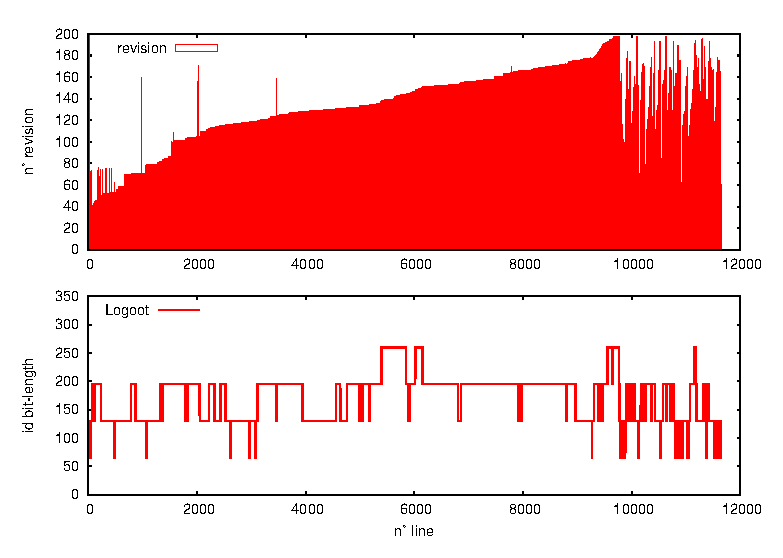
\includegraphics[width=0.48\textwidth]{./img/lseq/compliant.eps}}
  \hspace{10pt}
  \subfloat[Comportement d'édition inattendu]
  [\label{fig:lseq:motivating}Le comportement d'édition va à l'encontre des attentes
  de la stratégie d'allocation]
  {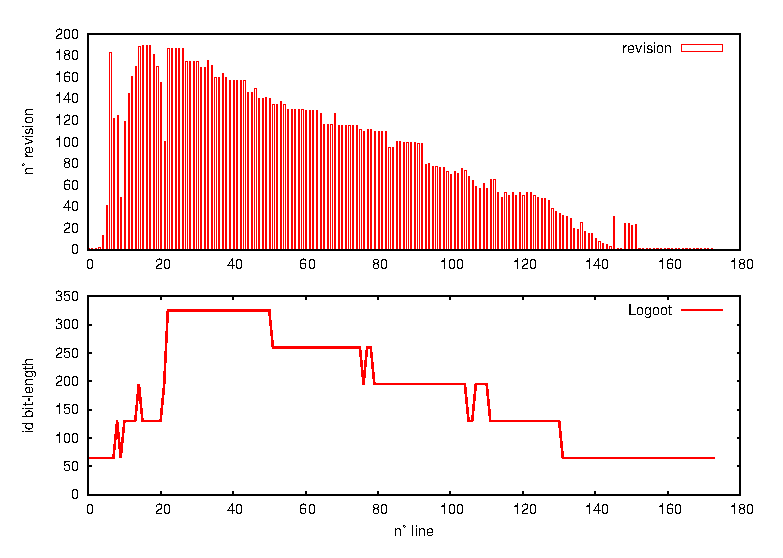
\includegraphics[width=0.48\textwidth]{./img/lseq/motivating.eps}}
  \caption{\label{fig:lseq:allocation}Spectre de documents Wikipedia sous différent
    comportements d'édition antagonistes. La figure du haut représente la
    révision à laquelle la ligne a été insérée, i.e., sa date de naissance.  La
    figure du bas représente la taille de l'identifiant associé à chaque ligne.}
\end{figure*}

Les figures~\ref{fig:lseq:compliant} et~\ref{fig:lseq:motivating} montrent deux
comportements d'éditions présent sur des pages extraites de Wikipedia. La partie
supérieure de ces figures donne une vue globale du comportement d'édition sur la
page. Elle indique la numéro de la révision à laquelle une ligne a été
insérée. Ainsi, plus une barre est haute, plus la ligne a été insérée
récemment. Le spectre de la figure~\ref{fig:lseq:compliant} montre que les
nouveaux éléments de la séquence sont principalement ajoutés en fin. À l'opposé,
le spectre de la figure~\ref{fig:lseq:motivating} montre que les nouveaux
éléments de la séquence sont principalement ajoutés en tête. La partie
inférieure de ces figures montre la taille de la représentation binaire de
l'identifiant associé à chaque élément du document. \TODO{Présenter la stratégie
  d'allocation}. Ainsi, nous observons que les identifiants dans le document
comportant 12k lignes mais principalement édité en fin a des identifiants
n'excédant pas 256 bits. En revanche, le document possédant seulement 170 lignes
édité en tête a des identifiants atteignant déjà les 320 bits.

\TODO{Définition du problème}

%%% Local Variables:
%%% mode: latex
%%% TeX-master: "../../paper"
%%% End:

%%
\section{LSEQ : une stratégie d'allocation polylogarithmique}

\LSEQ (abréviation pour \emph{polyLogarithimic SEQuence}) est une stratégie
d'allocation d'identifiants dont la taille est variable à la génération. Pour
générer ses identifiants immuables et uniques, \LSEQ utilise un arbre
exponentiel comme structure de données, deux sous-stratégies d'allocations avec
objectifs antagonistes, et un composant permettant de choisir la stratégie.

\subsection{Principe général}

Le principe général de \LSEQ consiste à amortir les mauvais choix d'identifiants
par un ensemble suffisant d'identifiants dont la taille est
satisfaisante. Puisqu'il n'existe pas de stratégie d'allocation parfaite sans
connaissance préalable de la séquence d'édition, \LSEQ cherche a être assez
général pour gérer la plupart des comportements d'édition.


\subsection{Arbre exponentiel}

Un arbre exponentiel est une structure d'arbre dont chaque élément de l'arbre
possède k-fois plus de fils que son parent. Par exemple, si l'on fixe $k$ à $2$,
un élément dont le parent possède $4$ fils en possède $8$. Dans ce cas, il y a
une augmentation quadratique du nombre de fils en fonction de la profondeur qui
s'ajoute à l'augmentation commune de l'arbre.

\TODO{figure}

Un identifiant \LSEQ est un suite d'entiers représentant le chemin de l'élément
dans l'arbre. Pour encoder cette suite d'entiers


\subsection{Sous-stratégies d'allocation}

\subsection{Choix de stratégie}

%%% Local Variables:
%%% mode: latex
%%% TeX-master: "../../paper"
%%% End:

%%
\section{Experimentations}

\subsection{Simulations}

%%% Local Variables:
%%% mode: latex
%%% TeX-master: "../../paper"
%%% End:

%%
\section{Conclusion}
\label{lseq:sec:conclusion}

%%% Local Variables:
%%% mode: latex
%%% TeX-master: "../../paper"
%%% End:


%%% Local Variables:
%%% mode: latex
%%% TeX-master: "../../paper"
%%% End:

% 
\chapter{Protocole d'échantillonnage aléatoire de pairs}

\minitoc


\section{Introduction}

\subsection{Champs d'applications}

\subsubsection{Dissémination d'informations}
\subsubsection{Gestion de topologies réseau}

\subsection{WebRTC}

\subsubsection{Facilité d'accès}
\subsubsection{Contraintes supplémentaires}


%%% Local Variables:
%%% mode: latex
%%% TeX-master: "../../paper"
%%% End:


\section{État de l'art}

\subsection{Voisinages à taille fixe}

\subsection{Éstimateurs de taile réseau}

\subsection{Voisinages à taille variable}

%%% Local Variables:
%%% mode: latex
%%% TeX-master: "../../paper"
%%% End:


\section{Spray : un protocole d'échantillonnage adaptatif}

\SPRAY est un protocole d'échantillonnage de paris adaptatif inspiré à la fois
de \SCAMP~\cite{ganesh2003peer} et \CYCLON~\cite{voulgaris2005cyclon}. \SPRAY
comprend trois parties représentant le cycle de vie d'un pair dans le
réseau. Tout d'abord, le processus consistant à rejoindre le réseau, qui injecte
un nombre logarithmique d'arcs comparé à la taille du réseau. De ce fait, le
nombre d'arcs passe à l'échelle. Ensuite, chaque pair éxecute un processus
periodique dont le but est d'équilibrer les vues partielles en termes de taille
et d'uniformité sur les pairs références dans celles-ci. Le réseau converge
rapidement vers une topologie possédant des propriétés similaires à celles des
graphes aléatoires. Enfin, un pair est capable de quitter le réseau à n'importe
quel moment sans en notifier le réseau (l'équivalent d'un crash) sans dégrader
les propriétés du reste du réseau.

L'obtention de cette propriété d'adaptivité repose essentiellement sur le fait
de conserver un nombre d'arcs cohérent durant tout le cycle de vie du réseau.
En effet, en opposition à \CYCLON, \SPRAY est toujours à la limite du nombre
optimal d'arcs. Comme \SPRAY n'ajoute jamais d'arcs après le processus d'entrée,
toute suppression d'arcs est définitive et ne doit donc pas être pris à la
légère. Ainsi, \SPRAY ajoute des arcs dans un premier temps. Dans un second
temps, le processus periodique de mélange des arcs de \SPRAY préserve tous les
arcs du réseau.  Dans un troisième temps, le processus de sortie supprime
précautionneusement quelques arcs. Dans l'idéal, il s'agit du nombre d'arcs
ajouté par le dernier pair entré dans le réseau.

Parfois, conserver le nombre d'arcs global constant force les processus de
mélange et de sortie à créer des doublons dans les vues partielles. Ainsi, une
vue partielle peut contenir plusieurs fois le même voisin. Toutefois, ces
doublons restent peu nombreux, et de ce fait, n'ont pas d'impact notable sur la
connectivité du réseau.

\subsection{Rejoindre le réseau}

L'algorithme pour rejoindre le réseau est, dans \SPRAY, la seule manière
d'introduire de nouveaux arcs dans le réseau. Afin de répondre à la première
partie de l'énoncé du problème (REF), ce nombre d'arcs doit augmenter
logarithmiquement comparé à la taille du réseau. Tout comme dans \SCAMP, nous
supposons que chacuns des pairs respecte cette contrainte. Dès lors, ces
derniers utilisent ce savoir afin de propager l'identité du nouvel
arrivant. L'algorithme~\ref{algo:joining} décrit la façon dont le contact envoie
la nouvelle identité à son voisinage où elle est intégrée directement à leur vue
partielle. En définitive, le nombre d'arcs dans le réseau augmente de
$1+\ln(|\mathcal{N}|)$ et ce, seulement en utilisant des interactions de voisin
à voisin.

\begin{figure*}
  \centering
  \subfloat[Figure A][$p_1$ contacts $p_2$ to join the network. $p_1$ adds
  $p_2$ to its neighborhood. $p_1$ sends its request to $p_2$.]{
    
\begin{tikzpicture}[scale=1.2]

  \newcommand\X{35pt};
  \newcommand\Y{15pt};

  \draw(-0.75*\X, 0pt); %% positioning
  \draw( 2.75*\X, 0pt); %% positioning

  \scriptsize
  \draw[->,dashed,very thick](5+0*\X, 0*\Y) -- 
  node[anchor=south]{(a)}(-5+ 2*\X, 0*\Y);
  \draw[->] (-5+2*\X, 5pt) -- (5+\X, \Y);
  \draw[->] (-5+2*\X, 5pt) --  (5+\X, 2*\Y);
  \draw[->] (-5+2*\X, -5pt) -- (5+\X, -\Y);
  \draw[->] (-5+2*\X, -5pt) -- (5+\X, -2*\Y);

  \draw[fill=white, very thick]
  (0*\X, 0*\Y) node{$p_1$} +(-5pt,-5pt) rectangle +(5pt,5pt);
  \draw[fill=white, very thick]
  (2*\X, 0*\Y) node{$p_2$} +(-5pt,-5pt) rectangle +(5pt,5pt);

  \draw[fill=white](1*\X,2*\Y) node{$p_6$} +(-5pt,-5pt) rectangle +(5pt,5pt);
  \draw[fill=white](1*\X,1*\Y) node{$p_5$} +(-5pt,-5pt) rectangle +(5pt,5pt);
  \draw[fill=white](1*\X,-1*\Y) node{$p_4$} +(-5pt,-5pt) rectangle +(5pt,5pt);
  \draw[fill=white](1*\X,-2*\Y) node{$p_3$} +(-5pt,-5pt) rectangle +(5pt,5pt);
  
\end{tikzpicture}}
  \hspace{8pt}
  \subfloat[Figure B][The $onSubs(p_1)$ event is raised at $p_1$
  which forwards the subscription to $p_1$'s neighborhood.]{
    
\begin{tikzpicture}[scale=1]

  \newcommand\X{35pt};
  \newcommand\Y{15pt};

  \draw(-0.75*\X, 0pt); %% positioning
  \draw( 2.75*\X, 0pt); %% positioning

  \scriptsize
  \draw[->](5+0*\X, 0*\Y) -- (-5+ 2*\X, 0*\Y);
  \draw[->, very thick] (-5+2*\X, 5pt) -- (5+\X, \Y);
  \draw[->, very thick] (-5+2*\X, 5pt) --
  node[anchor=south west]{(b)} (5+\X, 2*\Y);
  \draw[->, very thick] (-5+2*\X, -5pt) -- (5+\X, -\Y);
  \draw[->, very thick] (-5+2*\X, -5pt) --
  node[anchor=north west]{(b)}(5+\X, -2*\Y);

  \normalsize
  \draw[fill=white]
  (0*\X, 0*\Y) node{$p_1$} +(-5pt,-5pt) rectangle +(5pt,5pt);
  \draw[fill=white, very thick]
  (2*\X, 0*\Y) node{$p_2$} +(-5pt,-5pt) rectangle +(5pt,5pt);

  \draw[fill=white, very thick]
  (1*\X,2*\Y) node{$p_6$} +(-5pt,-5pt) rectangle +(5pt,5pt);
  \draw[fill=white, very thick]
  (1*\X,1*\Y) node{$p_5$} +(-5pt,-5pt) rectangle +(5pt,5pt);
  \draw[fill=white, very thick]
  (1*\X,-1*\Y) node{$p_4$} +(-5pt,-5pt) rectangle +(5pt,5pt);
  \draw[fill=white, very thick]
  (1*\X,-2*\Y) node{$p_3$} +(-5pt,-5pt) rectangle +(5pt,5pt);

\end{tikzpicture}}
  \hspace{8pt}
  \subfloat[Figure C][The $onFwdSubs(p_1)$ event is raised at $p_{3-6}$. The
  peers add $p_1$ to their neighborhood.]{
    
\begin{tikzpicture}[scale=1]

  \newcommand\X{35pt};
  \newcommand\Y{15pt};

  \draw(-0.75*\X, 0pt); %% positioning
  \draw( 2.75*\X, 0pt); %% positioning

  \scriptsize
  \draw[->](5+0*\X, 0*\Y) -- (-5+ 2*\X, 0*\Y);
  \draw[->] (-5+2*\X, 5pt) -- (5+\X, \Y);
  \draw[->] (-5+2*\X, 5pt) -- (5+\X, 2*\Y);
  \draw[->] (-5+2*\X, -5pt) -- (5+\X, -\Y);
  \draw[->] (-5+2*\X, -5pt) -- (5+\X, -2*\Y);

  \draw[->,dashed, very thick](-5+\X, 2*\Y) --
  node[anchor=south east]{(c)} ( 5pt,5pt);
  \draw[->,dashed, very thick](-5+\X, 1*\Y) -- ( 5pt,5pt);
  \draw[->,dashed, very thick](-5+\X, -1*\Y) -- ( 5pt,-5pt);
  \draw[->,dashed, very thick](-5+\X, -2*\Y) --
  node[anchor=north east]{(c)}( 5pt,-5pt);

  \normalsize
  \draw[fill=white, very thick]
  (0*\X, 0*\Y) node{$p_1$} +(-5pt,-5pt) rectangle +(5pt,5pt);
  \draw[fill=white]
  (2*\X, 0*\Y) node{$p_2$} +(-5pt,-5pt) rectangle +(5pt,5pt);

  \draw[fill=white, very thick]
  (1*\X,2*\Y) node{$p_6$} +(-5pt,-5pt) rectangle +(5pt,5pt);
  \draw[fill=white, very thick]
  (1*\X,1*\Y) node{$p_5$} +(-5pt,-5pt) rectangle +(5pt,5pt);
  \draw[fill=white, very thick]
  (1*\X,-1*\Y) node{$p_4$} +(-5pt,-5pt) rectangle +(5pt,5pt);
  \draw[fill=white, very thick]
  (1*\X,-2*\Y) node{$p_3$} +(-5pt,-5pt) rectangle +(5pt,5pt);
 

\end{tikzpicture}}
  \caption{\label{fig:joiningexample}Example of the \SPRAY's joining
    protocol.}
\end{figure*}

\begin{algorithm}

\small
\algrenewcommand{\algorithmiccomment}[1]{\hskip2em$\rhd$ #1}

\newcommand{\comment}[1]{$\rhd$ #1}


\algblockdefx[initially]{initially}{endInitially}
  [0] {\textbf{INITIALLY:}} 

\algblockdefx[pas]{pas}{endPas}
  [0] {\textbf{EVENTS:}}

\newcommand{\LINEFOR}[2]{%
  \algorithmicfor\ {#1}\ \algorithmicdo\ {#2} %
  }

\newcommand{\LINEIFTHEN}[2]{%
  \algorithmicif\ {#1}\ \algorithmicthen\ {#2} %
  }

\newcommand{\INDSTATE}[1][1]{\State\hspace{\algorithmicindent}}

\begin{algorithmic}[1]
  \Statex
  \initially
    \State $\mathcal{P} \leftarrow \varnothing$;
    \hfill \comment{the partial view is a multiset}
    \State $p$ ; \hfill \comment{identity of the local peer}
  \endInitially
  
  \pas
  \Function{onSubs}{$o$} \hfill \comment{$o: origin$}
    \State \LINEFOR{\textbf{each} $\langle q,\,\_\, \rangle \in\mathcal{P}$}
    {$sendTo(q,\, 'fwdSubs',\, o)$;} \label{line:multicast}
    \EndFunction
    \Statex
    \Function{onFwdSubs}{$o$} \hfill \comment{$o: origin$}
    \State $\mathcal{P} \leftarrow
    \mathcal{P}\uplus \left\{\langle o,\, 0 \rangle\right\}$;
    \EndFunction
  \endPas
  
\end{algorithmic}

\caption{\label{algo:joining}The joining protocol of \SPRAY.}
\end{algorithm}

La vue partielle est un multiensemble de couples $\langle n,\, age\rangle$ qui
associe à chaque voisin $n$ l'âge $age$. Ce multiensemble permet de gérer les
doublons. L'âge joue le même rôle que dans \CYCLON, çàd qu'il accélère la
suppression des pairs qui sont sortis ou ont crash. L'évenement $onSubs$ est
appelé chaque fois qu'un pair rejoins le réseau via ce contact. $onSubs$
redirige l'identité du pairs à tous ses voisins, indépendament de
l'âge. L'évenement $onFwdSubs$ est déclanché lorsqu'un pair reçoit une telle
identité redirigée. $onFwdSubs$ ajoute la référence en initialisant son âge à
$0$.

La figure~\ref{fig:joiningexample} décrit un scenario où le pair $p_1$ contacte
le pair $p_2$ afin de rejoindre le réseau composé de $\{p_2$, $p_2$, $p_4$,
$p_5$, $p_6\}$. Pour simplifier, la figure ne montre que les arcs nouvellement
introduit ainsi que le voisinage de $p_1$ et $p_2$. Le pair $p_1$ ajoute
directement $p_2$ dans sa vue partielle. Ce dernier redirige l'identité de $p_1$
à chacun de ses voisins.  Chacun de ces voisins ajoute alors $p_1$ à leur vue
partielle. Au total, \SPRAY établie 5 connexions. Le réseau en résultant est
connecté.

Malheureusement, les vues partiels des derniers arrivant sont clairement
déséquilibrés comparé au reste du réseau. De ce fait, ils violent la première
condition de l'énoncé du problème (REF). Le processus de mélange décrit dans la
prochaine section a pour but de ré-équilibrer les vues partielles.

\subsection{Échanger son voisinage}

Au contraire de \CYCLON, \SPRAY mélange des vues partielles dont les tailles
peuvent être différentes. Ce processus à pour but d'équilibrer les tailles de
vue partielles ainsi que de mélanger les références à l'interieur de celles-ci.
Ce processus à pour contrainte de conserver l'exact même nombre d'arcs.

Les deux pairs impliqués dans le mélange s'envoient l'un l'autre la moitié de
leur vue partielle. Après l'intégration de ces nouvelles références, la taille
de leur vue partielle tend vers la moyenne, et la somme globale en demeure
inchangée. Dans ce but, les vues partielles sont des multiensembles. Ainsi, si
un pair réçoit une référence déjà connue, il la conserve en tant que doublon.
De cette façon, le nombre d'arcs reste constant.

Si les doublons ont un impact négatif sur les propriétés du réseau, la plupart
de ceux-ci disparaissent après le processus de mélange. En proportion, ils
deviennent négligeable dès lors que le réseau grandit.

\begin{algorithm}[h]
  
\small
\algrenewcommand{\algorithmiccomment}[1]{\hskip2em$\rhd$ #1}

\newcommand{\comment}[1]{$\rhd$ #1}

\algblockdefx[act]{act}{endAct}
  [0] {\textbf{ACTIVE THREAD:}}

\algblockdefx[pas]{pas}{endPas}
  [0] {\textbf{PASSIVE THREAD:}}


\newcommand{\LINEFOR}[2]{%
  \algorithmicfor\ {#1}\ \algorithmicdo\ {#2} %
  }

\newcommand{\LINEIFTHEN}[2]{%
  \algorithmicif\ {#1}\ \algorithmicthen\ {#2} %
  }

\newcommand{\INDSTATE}[1][1]{\State\hspace{\algorithmicindent}}

\begin{algorithmic}[1]
  \Statex
  \act
    \Function{loop}{ } \hfill \comment{Every $\Delta\,t$}
    \State $\mathcal{P} \leftarrow incrementAge(\mathcal{P})$;
    \State \textbf{let} $ \langle q,\, age \rangle \leftarrow getOldest(\mathcal{P})$;
    \State \textbf{let} $sample \leftarrow $ \label{line:samplesize}
    $getSample(\mathcal{P}\setminus\left\{\langle q, age\rangle\right\}, \left \lceil{|\mathcal{P}|\over{2}} \right \rceil-1) \uplus \left\{\langle p, 0 \rangle\right\}$;
    \State $sample \leftarrow replace(sample,\,q,\,p)$; \label{line:replace1}
    \State $sendTo(q,\, 'exchange',\, sample)$;
    \State \textbf{let} $sample'\leftarrow receiveFrom(q)$;
    \State $sample \leftarrow replace(sample,\,p,\,q)$;
    \State $\mathcal{P} \leftarrow (\mathcal{P} \setminus sample) \uplus
    sample'$;
    \EndFunction
  \endAct
  
  \pas
    \Function{onExchange}{$o,\, sample$} \hfill \comment{$o: origin$}
    \State \textbf{let} $sample' \leftarrow getSample(\mathcal{P} ,\, \left\lceil |\mathcal{P}|\over{2} \right\rceil )$;
    \State $sample' \leftarrow replace(sample',\,o,\,p);$ \label{line:replace2}
    \State $sendTo(o ,\, sample')$;
    \State $sample' \leftarrow replace(sample',\,p,\,o)$;
    \State $\mathcal{P} \leftarrow (\mathcal{P} \setminus sample') \uplus
    sample$; 
    \EndFunction
  \endPas
  
\end{algorithmic}

  \caption{\label{algo:scamplon}The cyclic protocol of \SPRAY.}
\end{algorithm}

L'algorithme~\ref{algo:scamplon} montre la partie periodic de \SPRAY éxécutée
par chaque pair. Il est divisé en deux parties, à savoir le processus actif qui
est appelé régulièrement afin d'initier un mélange de vues, et le processus
passif qui réagit au message du processus actif. Les fonctions qui ne sont pas
explicitement définies sont les suivantes:
\begin{compactitem}
\item $incrementAge(view)$ : incrémente l'âge des éléments présent dans la vue
  $view$ et retourne la vue modifiée.
\item $getOldest(view)$ : retourne le plus vieu des pairs présent dans la vue.
\item $getSample(view,\, size)$ : retourne un échantillon de la vue contenant $size$
  éléments.
\item $replace(view,\,old,\,new)$ : remplace les occurrences de $old$ par $new$ dans
  la vue $view$.
\item $rand()$ : retourne un nombre flottant aléatoire entre $0$ et $1$.
\end{compactitem}

Dans le processus actif, la fonction $loop$ est appelée tous les intervals
$\Delta$ de temps. Tout d'abord, la fonction incrémente l'age de chacun des
voisins dans la vue partielle $\mathcal{P}$. Ensuite, le pair le plus âgé $q$
est choisit afin d'initier un échange. Si le pair $q$ ne peut être joint (car il
est parti ou a crash), alors le pair $p$ éxecute la fonction qui gère ce cas
(voir la section suivante). Ceci est répété jusqu'à ce que $p$ trouve un pair
avec qui communiquer. Ainsi, le vieillissement comme héritage de \CYCLON permet
d'accélérer la suppression des références invalides. Une fois que le pair
initiateur $p$ a trouvé un pair avec qui effectuer l'échange, il selectionne un
échantillon de sa vue partielle tout en excluant la référence à $q$ et en
s'incluant lui-même. La taille de l'échantillon correspond à la moitié de la
taille de la vue partielle avec au minimum $1$ pair : sa propre référence
(cf. Line~\ref{line:samplesize}). La réponse de $q$ contient également la moitié
de sa vue partielle. Puisque les pairs ne peuvent apparaitre plusieurs fois dans
$\mathcal{P}$, les pairs impliqués dans le processus d'échange peuvent envoyer
des références cet autre pair ($p$ envoie des références $q$ à $q$). Sans
procédures supplémentaires, ce genre de comportement peut créer des boucles
locales ($q$ a $q$ dans sa vue partielle) ce qui est hautement indésirable. Les
lignes~\ref{line:replace1},~\ref{line:replace2} permettent de remplacer les
auto-références dans l'échantillon. Enfin, chez les deux pairs, l'échantillon envoyé 
est supprimé de la vue partielle, et l'échantillon réçu est ajouté.

\begin{figure*}
  \centering
  \subfloat[Figure A]
  [Peer $p_6$ initiates the exchange with $p_1$ by sending to the
  latter the multiset $\{p_6,\,p_9\}$.]{
    
\begin{tikzpicture}[scale=1.2]

  \newcommand\X{35pt};
  \newcommand\Y{15pt};

  \draw[->](5+0*\X, 0*\Y) -- (-5+ 2*\X, 0*\Y); %% 1 -> 2
  \draw[->] (-5+2*\X, 5pt) -- (5+\X, \Y);
  \draw[->](2*\X,5pt) -- (5+1*\X, 2*\Y); %% 2 -> 6
  \draw[->] (-5+2*\X, -5pt) -- (5+\X, -\Y);
  \draw[->] (-5+2*\X, -5pt) -- (5+\X, -2*\Y);

  \draw[->,very thick](-5+\X,2*\Y) -- (0pt,5pt); %% 6 -> 1

  \draw[->](-5+\X, 1*\Y) -- ( 5pt,5pt);
  \draw[->](-5+\X, -1*\Y) -- ( 5pt,-5pt);
  \draw[->](-5+\X, -2*\Y) -- ( 5pt,-5pt);

  \draw[->](-5+\X, 5+2*\Y)to[out=120,in=30](0pt,5+2*\Y); %% 6 -> 7
  \draw[->](-5+\X, 5+2*\Y)to[out=120,in=30](-5-\Y ,5+2*\Y); %% 6 -> 8
  \draw[->](-5+\X, 5+2*\Y)to[out=120,in=30](-10-2*\Y,5+2*\Y); %% 6 -> 9

  \normalsize
  \draw[fill=white, very thick]
  (0*\X, 0*\Y) node{$p_1$} +(-5pt,-5pt) rectangle +(5pt,5pt);
  \draw[fill=white](2*\X, 0*\Y) node{$p_2$} +(-5pt,-5pt) rectangle +(5pt,5pt);

  \draw[fill=white,very thick]
  (1*\X,2*\Y) node{$\mathbf{p_6}$} +(-5pt,-5pt) rectangle +(5pt,5pt);
  \draw[fill=white](1*\X,1*\Y) node{$p_5$} +(-5pt,-5pt) rectangle +(5pt,5pt);
  \draw[fill=white](1*\X,-1*\Y) node{$p_4$} +(-5pt,-5pt) rectangle +(5pt,5pt);
  \draw[fill=white](1*\X,-2*\Y) node{$p_3$} +(-5pt,-5pt) rectangle +(5pt,5pt);

  \draw[fill=white]( 0*\X,2*\Y)
  node{$p_7$} +(-5pt,-5pt) rectangle +(5pt,5pt);
  \draw[fill=white](-5+-\Y,2*\Y)node{$p_8$} +(-5pt,-5pt) rectangle +(5pt,5pt);
  \draw[fill=white](-10+-2*\Y,2*\Y) node{$\mathbf{p_9}$} +(-5pt,-5pt) rectangle +(5pt,5pt);
  

\end{tikzpicture}}
  \hspace{10pt}
  \subfloat[Figure B][Peer $p_1$ receives the $p_6$'s message. 
  It sends back the multiset $\{p_2\}$ and adds $\{p_6,\,p_9\}$ to its 
  partial view.]{
    
\begin{tikzpicture}[scale=1.2]

  \newcommand\X{35pt};
  \newcommand\Y{15pt};

  \draw[->](5+0*\X, 0*\Y) -- (-5+ 2*\X, 0*\Y); %% 1 -> 2
  \draw[->] (-5+2*\X, 5pt) -- (5+\X, \Y);
  \draw[->](2*\X,5pt) -- (5+1*\X, 2*\Y); %% 2 -> 6
  \draw[->] (-5+2*\X, -5pt) -- (5+\X, -\Y);
  \draw[->] (-5+2*\X, -5pt) -- (5+\X, -2*\Y);

  \draw[->,dashed, very thick](0pt,5pt)--(-5+\X, 2*\Y); %% 1 -> 6

  \draw[->](-5+\X, 1*\Y) -- ( 5pt,5pt);
  \draw[->](-5+\X, -1*\Y) -- ( 5pt,-5pt);
  \draw[->](-5+\X, -2*\Y) -- ( 5pt,-5pt);

  \draw[->](-5+\X, 5+2*\Y)to[out=120,in=30](0pt,5+2*\Y); %% 6 -> 7
  \draw[->](-5+\X, 5+2*\Y)to[out=120,in=30](-5-\Y ,5+2*\Y); %% 6 -> 8
  
  \draw[->,dashed, very thick](-5pt,5pt)--(-10-2*\Y,-5+2*\Y); %% 1 -> 9

  \normalsize
  \draw[fill=white, very thick]
  (0*\X, 0*\Y) node{$p_1$} +(-5pt,-5pt) rectangle +(5pt,5pt);
  \draw[fill=white](2*\X, 0*\Y)
  node{$\mathbf{p_2}$} +(-5pt,-5pt) rectangle +(5pt,5pt);

  \draw[fill=white,very thick]
  (1*\X,2*\Y) node{$p_6$} +(-5pt,-5pt) rectangle +(5pt,5pt);
  \draw[fill=white](1*\X,1*\Y) node{$p_5$} +(-5pt,-5pt) rectangle +(5pt,5pt);
  \draw[fill=white](1*\X,-1*\Y) node{$p_4$} +(-5pt,-5pt) rectangle +(5pt,5pt);
  \draw[fill=white](1*\X,-2*\Y) node{$p_3$} +(-5pt,-5pt) rectangle +(5pt,5pt);

  \draw[fill=white]( 0*\X,2*\Y)
  node{$p_7$} +(-5pt,-5pt) rectangle +(5pt,5pt);
  \draw[fill=white](-5+-\Y,2*\Y)node{$p_8$} +(-5pt,-5pt) rectangle +(5pt,5pt);
  \draw[fill=white](-10+-2*\Y,2*\Y) node{$p_9$} +(-5pt,-5pt) rectangle +(5pt,5pt);
  

\end{tikzpicture}}
  \hspace{10pt}
  \subfloat[Figure C][Peer $p_6$ receives the $p_1$'s response, it
  adds $\{p_2\}$ to its partial view.]{
    
\begin{tikzpicture}[scale=1.2]

  \newcommand\X{35pt};
  \newcommand\Y{15pt};

  \draw[->] (-5+2*\X, 5pt) -- (5+\X, \Y);
  \draw[->,dashed, very thick]
  (5+\X, 2*\Y)to[out=-20,in=110](2*\X, 5pt); %% 6 -> 2
  \draw[->](2*\X,5pt)to[out=160,in=-70](5+1*\X, 2*\Y); %% 2 -> 6
  \draw[->] (-5+2*\X, -5pt) -- (5+\X, -\Y);
  \draw[->] (-5+2*\X, -5pt) -- (5+\X, -2*\Y);

  \draw[->](0pt,5pt)--(-5+\X, 2*\Y); %% 1 -> 6

  \draw[->](-5+\X, 1*\Y) -- ( 5pt,5pt);
  \draw[->](-5+\X, -1*\Y) -- ( 5pt,-5pt);
  \draw[->](-5+\X, -2*\Y) -- ( 5pt,-5pt);

  \draw[->](-5+\X, 5+2*\Y)to[out=120,in=30](0pt,5+2*\Y); %% 6 -> 7
  \draw[->](-5+\X, 5+2*\Y)to[out=120,in=30](-5-\Y ,5+2*\Y); %% 6 -> 8
  
  \draw[->](-5pt,5pt)--(-10-2*\Y,-5+2*\Y); %% 1 -> 9

  \normalsize
  \draw[fill=white]
  (0*\X, 0*\Y) node{$p_1$} +(-5pt,-5pt) rectangle +(5pt,5pt);
  \draw[fill=white](2*\X, 0*\Y) node{$p_2$} +(-5pt,-5pt) rectangle +(5pt,5pt);

  \draw[fill=white,very thick]
  (1*\X,2*\Y) node{$p_6$} +(-5pt,-5pt) rectangle +(5pt,5pt);
  \draw[fill=white](1*\X,1*\Y) node{$p_5$} +(-5pt,-5pt) rectangle +(5pt,5pt);
  \draw[fill=white](1*\X,-1*\Y) node{$p_4$} +(-5pt,-5pt) rectangle +(5pt,5pt);
  \draw[fill=white](1*\X,-2*\Y) node{$p_3$} +(-5pt,-5pt) rectangle +(5pt,5pt);

  \draw[fill=white]( 0*\X,2*\Y)
  node{$p_7$} +(-5pt,-5pt) rectangle +(5pt,5pt);
  \draw[fill=white](-5+-\Y,2*\Y)node{$p_8$} +(-5pt,-5pt) rectangle +(5pt,5pt);
  \draw[fill=white](-10+-2*\Y,2*\Y) node{$p_9$} +(-5pt,-5pt) rectangle +(5pt,5pt);
  

\end{tikzpicture}}
  \caption{\label{fig:spray:cyclicexample}Example of the \SPRAY's shuffling
    protocol. }
\end{figure*}

La figure~\ref{fig:spray:cyclicexample} décrit le méchanisme périodique de \SPRAY. Ce
scénario suit celui de la figure~\ref{fig:joiningexample}: le pair $p_1$ vient
de rejoindre le réseau. Le pair $p_6$ initie un échange avec $p_1$ (qui est ici
le plus vieux dans sa vue partielle). $p_6$ choisit
$\left\lceil{|\mathcal{P}_6|\div 2}\right\rceil = 1$ aléatoirement parmis son
voisinnage. Dans ce cas, il choisit $p_9$ parmis $\{p_9,\,p_8,\,p_7\}$. Il
envoie à $p_1$ cet échantillon auquel est ajoutée sa propre identité. En
réponse, le pair $p_1$ choisit
$\left\lceil{|\mathcal{P}_1|\div 2}\right\rceil = 1$ pair de sa vue
partielle. L'échantillon composé du seul voisin $p_2$ est envoyé. Immédiatement
après, $p_1$ peut supprimer l'échantillon envoyé et intégrer celui réçu
résultant en une vue partielle composée de $\{p_6,\, p_9\}$. De la même façon,
après réception de l'échantillon de $p_1$, $p_6$ supprime et intègre les
échantillons adéquats, résultant en une vue partielle composée de
$\{p_2,\,p_7,\,p_8\}$.

La procédure d'échange tend à réduire l'écart de taille des vues partielles. De
plus, elle disperse les références aux pairs afin de supprimer les groupes trop
denses dûes à la procédure d'entrée dans le réseau.

En ce qui concerne le temps de converge de l'algorithme de mélange, il existe
une relation proche entre \SPRAY et le protocole d'aggrégation proactive
présenté dans~\cite{jelasity2004epidemic, montresor2004robust}. Celui-ci déclare
que, sous l'hypothèse d'un échantillonnage suffisamment aléatoire, la valeur
moyenne $\mu$ et la variance $\sigma^2$ a un cycle $i$ sont :
\begin{center}
  $\mu_i = {1\over{|\mathcal{N}|}} \sum\limits_{x \in \mathcal{N}} a_{i,\,x}$
  \hfill
  $\sigma^2_i = {1\over{|\mathcal{N}|-1}}\sum\limits_{x \in \mathcal{N}}
  (a_{i,\,x} - \mu_i)^2$
\end{center}
avec $a_{i,\,x}$ la valeur stockée par le pair $p_x$ au cycle $i$. La variance
estimée doit converger en 0 au cours des cycles. En d'autres termes, les valeurs
se rapprochent les unes des autres au cours des cycles. Dans le cas de \SPRAY,
cette valeur $a_{i,\,x}$ est la taille de la vue partiel du pair $p_x$ au cycle
$i$. En effet, chaque échange du pair $p_1$ et du pair $p_2$ est une aggrégation
dont le résultat est :
$|\mathcal{P}_1|\approx|\mathcal{P}_2|\approx{(|\mathcal{P}_1| +
  |\mathcal{P}_2|) \div 2}$.
De plus, à chaque cycle, chaque pair est impliqué dans un protocole d'échange au
moins une fois (celui qu'ils initient), and, dans le meilleur des cas
$1+Poisson(1)$ (celui qu'ils initient et, en moyenne, celui qu'ils réçoivent
d'un autre pair). Cette relation étant établie, nous en déduisons que la taille
des vues partielles des pairs de \SPRAY converge en temps exponentiel vers la
moyenne globale. De plus, chaque cycle réduit la variance du système global à un
taux compris entre ${1\div 2}$ et $1\div ({2\sqrt{\text{e}}})$.

\subsection{Quitter le réseau}

Avec \SPRAY, les pairs peuvent quitter le réseau sans alerter qui que ce
soit. Nous ne faisons pas de distinctions particulières entre les départs et les
crashs. Toutefois, le protocole doit réagir à ces deux cas. En effet, sans
réactions, le réseau pourrait s'éffondrer pour cause de suppression d'arcs trop
zélé. Lorsqu'un pair rejoint le réseau, il y injecte $1+\ln(|\mathcal{N}|)$
arcs. Néanmoins, après plusieurs échanges, la vue partielle du pair rejoignant
le réseau est remplie par d'autres références. Ainsi, quand il quitte le réseau,
il entraine la suppression de $\ln(|\mathcal{N}|)$ arcs de sa vue partielle, et
$\ln(|\mathcal{N}|)$ arcs des pairs l'ayant dans leur vue partielle. Par
conséquent, sans moyens de gérer les départs, $2\ln(\mathcal{N}|)$ arcs sont
supprimés au lieu des $1+\ln(|\mathcal{N}|)$. Afin d'y remedier, chaque pair qui
détecte un crash peut rétablir une connexion avec l'un de ces voisins en
introduisant un doublon (doublon qui disparaitra rapidement après quelques
protocoles d'échange). La probabilité de réétablir une connexion est
$1-1\div{|\mathcal{P}|}$. Puisque ${|\mathcal{P}|}\approx \ln(|\mathcal{N}|)$
pairs ont detecté le crash dans leur vue partielle, il est probable qu'ils
recréent tous la connexion perdue, à l'exception d'un pair. De ce fait,
lorsqu'un pair quitte le réseau, il entraine la suppression d'un nombre d'arcs
correspondant approximativement au nombre d'arcs ajouté lors de la dernière
entrée de pair.

\begin{algorithm}[h]
  
\small
\algrenewcommand{\algorithmiccomment}[1]{\hskip2em$\rhd$ #1}

\newcommand{\comment}[1]{$\rhd$ #1}

\newcommand{\LINEFOR}[2]{%
  \algorithmicfor\ {#1}\ \algorithmicdo\ {#2} %
  }

\newcommand{\LINEIFTHEN}[2]{%
  \algorithmicif\ {#1}\ \algorithmicthen\ {#2} %
  }

\newcommand{\INDSTATE}[1][1]{\State\hspace{\algorithmicindent}}

\begin{algorithmic}[1]
  \Function{onPeerDown}{$q$} \hfill \comment{$q$: crashed/departed peer}  
  \State \textbf{let} $occ \leftarrow 0$;

  \For{\textbf{each} $\langle n,\,age\rangle \in \mathcal{P}$}
  \hfill \comment{remove and count}
  \If {($n=q$)}
  \State $\mathcal{P} \leftarrow \mathcal{P}\setminus \{\langle n,\,age\rangle \}$;
  \State $occ \leftarrow occ + 1$;
  \EndIf
  \EndFor

  \For{$i\leftarrow 0$ \textbf{to} $occ$} 
  \hfill \comment{probabilistically duplicates}
  \If{($rand()>{1\over{|\mathcal{P}|+occ}}$)}
  \State \textbf{let} $\langle n,\,\_ \,\rangle \leftarrow
  \mathcal{P}[\left\lfloor rand()*|\mathcal{P}|\right\rfloor]$;
  \State $\mathcal{P} \leftarrow \mathcal{P} \uplus
  \left\{\langle n,\, 0\rangle\right\}$;
  \EndIf
  \EndFor
  
  \EndFunction
  \Statex
  \Function{onArcDown}{$q,\,age$}
  \hfill \comment{$q$: arrival of the arc down}  
  \State $\mathcal{P} \leftarrow \mathcal{P}\setminus \{\langle q,\,age\rangle \}$;
  \State \textbf{let} $\langle n,\,\_ \,\rangle \leftarrow
  \mathcal{P}[\left\lfloor rand()*|\mathcal{P}|\right\rfloor]$;
  \State $\mathcal{P} \leftarrow \mathcal{P} \uplus
  \left\{\langle n,\, 0\rangle\right\}$;
  \hfill \comment{systematically duplicates}
  \EndFunction

\end{algorithmic}

  \caption{\label{algo:unreachable}The crash/departure handler of \SPRAY.}
\end{algorithm}

L'algorithme~\ref{algo:unreachable} montre la manière selon laquelle \SPRAY gère
les départs et crashs. La fonction $onPeerDown$ montre la réaction de \SPRAY
lorsque le pair $q$ est detecté comme parti ou défaillant. Dans un premier
temps, la fonction compte les occurences du pair $q$ dans la vue partielle et
les supprimes. Dans un second temps, une boucle ajoute de manière probabiliste
des doublons de références à des pairs déjà connus. La probabilité dépend de la
taille de la vue partielle avant la suppression.

\begin{figure*}
  \centering
  \subfloat[Figure A][Peer $p_1$ crashes.]{
    
\begin{tikzpicture}[scale=0.9]

  \newcommand\X{35pt};
  \newcommand\Y{15pt};
  \large
  \draw[->](-5+\X, 1*\Y) --node{$\times$} ( 5pt,5pt);
  \draw[->](-5+\X, -1*\Y) --node{$\times$} ( 5pt,-5pt);
  \draw[->](-5+\X, -2*\Y) --node{$\times$} ( 5pt,-5pt);

  \draw[->](-5pt,5pt)--node{$\times$}(-10-2*\Y,-5+2*\Y); %% 1 -> 9
  \draw[->](-5pt,5pt)--node{$\times$}(-5-1*\Y,-5+2*\Y); %% 1 ->8 
  \draw[->](-5pt,5pt)--node{$\times$}(0pt,-5+2*\Y); %% 1 -> 7
  \draw[->](-5pt,5pt)--node{$\times$}(-5+\X,-5+2*\Y); %% 1 -> 6
  \normalsize
  \draw[->](5+ 1*\X, 5+ 1*\Y)--(-5+2*\X, 2*\Y); %% 5 -> 14
  \draw[->](5+1*\X,  1*\Y)--(-5+2*\X, 1*\Y); %% 5 -> 13 
  
  \draw[->](5+\X, 5-\Y) -- (-5+2*\X,0pt); %% 4 -> 12
  \draw[->](5+\X, -\Y) -- (-5+2*\X, -\Y); %% 4 -> 11
  
  \draw[->](5+\X, -2*\Y) -- (-5+2*\X, -2*\Y);
  
  \small
  \draw[fill=white,very thick]
  (0*\X, 0*\Y) node{$p_1$} +(-5pt,-5pt) rectangle +(5pt,5pt);
  \draw[thick] (-5pt,-5pt) -- (5pt,5pt);
  \draw[thick] (-5pt, 5pt) -- (5pt,-5pt);
  
  \draw[fill=white]
  (1*\X,1*\Y) node{$p_5$} +(-5pt,-5pt) rectangle +(5pt,5pt);
  \draw[fill=white]
  (1*\X,-1*\Y) node{$p_4$} +(-5pt,-5pt) rectangle +(5pt,5pt);
  \draw[fill=white]
  (1*\X,-2*\Y) node{$p_3$} +(-5pt,-5pt) rectangle +(5pt,5pt);

  \draw[fill=white](\X,2*\Y) node{$p_6$} +(-5pt,-5pt) rectangle +(5pt,5pt);

  \draw[fill=white]( 0*\X,2*\Y)
  node{$p_7$} +(-5pt,-5pt) rectangle +(5pt,5pt);
  \draw[fill=white](-5+-\Y,2*\Y)node{$p_8$} +(-5pt,-5pt) rectangle +(5pt,5pt);
  \draw[fill=white](-10+-2*\Y,2*\Y) node{$p_9$} +(-5pt,-5pt) rectangle +(5pt,5pt);
  
  \draw[fill=white](2*\X,2*\Y)node{$p_{14}$} +(-5pt,-5pt) rectangle +(5pt,5pt);
  \draw[fill=white](2*\X,1*\Y)node{$p_{13}$} +(-5pt,-5pt) rectangle +(5pt,5pt);
  \draw[fill=white](2*\X,0*\Y)node{$p_{12}$} +(-5pt,-5pt) rectangle +(5pt,5pt);
  \draw[fill=white](2*\X,-1*\Y)node{$p_{11}$}+(-5pt,-5pt) rectangle +(5pt,5pt);
  \draw[fill=white](2*\X,-2*\Y)node{$p_{10}$}+(-5pt,-5pt) rectangle +(5pt,5pt);

\end{tikzpicture}}
  \hspace{10pt}
  \subfloat[Figure B][The peers $p_{3-5}$ notice that they cannot
  reach $p_1$ anymore.]{
    
\begin{tikzpicture}[scale=0.9]

  \newcommand\X{35pt};
  \newcommand\Y{15pt};

  \large
  \draw[->, very thick](-5+\X, 1*\Y) -- node{$\times$} ( 5pt,5pt);
  \draw[->, very thick](-5+\X, -1*\Y) --node{$\times$} ( 5pt,-5pt);
  \draw[->, very thick](-5+\X, -2*\Y) --node{$\times$} ( 5pt,-5pt);

  \normalsize

  \draw[->](5+ 1*\X, 5+ 1*\Y)--(-5+2*\X, 2*\Y); %% 5 -> 14
  \draw[->](  5+1*\X, 1*\Y)--(-5+2*\X, 1*\Y); %% 5 -> 13 (v)
  
  \draw[->](5+\X, 5-\Y) -- (-5+2*\X,0pt); %% 4 -> 12
  \draw[->](5+\X, -\Y) -- (-5+2*\X, -\Y); %% 4 -> 11
  
  \draw[->](5+\X, -2*\Y) -- (-5+2*\X, -2*\Y);
  
  \small
  \draw[fill=white]
  (0*\X, 0*\Y) node{$p_1$} +(-5pt,-5pt) rectangle +(5pt,5pt);
  \draw (-5pt,-5pt) -- (5pt,5pt);
  \draw (-5pt, 5pt) -- (5pt,-5pt);
  
  \draw[fill=white, very thick]
  (1*\X,1*\Y) node{$p_5$} +(-5pt,-5pt) rectangle +(5pt,5pt);
  \draw[fill=white, very thick]
  (1*\X,-1*\Y) node{$p_4$} +(-5pt,-5pt) rectangle +(5pt,5pt);
  \draw[fill=white, very thick]
  (1*\X,-2*\Y) node{$p_3$} +(-5pt,-5pt) rectangle +(5pt,5pt);

  \draw[fill=white](\X,2*\Y) node{$p_6$} +(-5pt,-5pt) rectangle +(5pt,5pt);

  \draw[fill=white]( 0*\X,2*\Y)
  node{$p_7$} +(-5pt,-5pt) rectangle +(5pt,5pt);
  \draw[fill=white](-5+-\Y,2*\Y)node{$p_8$} +(-5pt,-5pt) rectangle +(5pt,5pt);
  \draw[fill=white](-10+-2*\Y,2*\Y) node{$p_9$} +(-5pt,-5pt) rectangle +(5pt,5pt);
  
  \draw[fill=white](2*\X,2*\Y)node{$p_{14}$} +(-5pt,-5pt) rectangle +(5pt,5pt);
  \draw[fill=white](2*\X,1*\Y)node{$p_{13}$} +(-5pt,-5pt) rectangle +(5pt,5pt);
  \draw[fill=white](2*\X,0*\Y)node{$p_{12}$} +(-5pt,-5pt) rectangle +(5pt,5pt);
  \draw[fill=white](2*\X,-1*\Y)node{$p_{11}$}+(-5pt,-5pt) rectangle +(5pt,5pt);
  \draw[fill=white](2*\X,-2*\Y)node{$p_{10}$}+(-5pt,-5pt) rectangle +(5pt,5pt);

\end{tikzpicture}}
  \hspace{10pt}
  \subfloat[Figure C][The peers $p_3$ and $p_5$ choose to establish
  a duplicate with one of their existing neighbor.]{
    
\begin{tikzpicture}[scale=1.2]

  \newcommand\X{35pt};
  \newcommand\Y{15pt};

  \draw[->](5+ 1*\X, 5+ 1*\Y)--(-5+2*\X, 2*\Y); %% 5 -> 14
  \draw[->](5+1*\X, 2.5+ 1*\Y)--(-5+2*\X, 2.5+ 1*\Y); %% 5 -> 13 (^)
  \draw[->,dashed, very thick]
  (  5+1*\X,-2.5+1*\Y)--(-5+2*\X,-2.5+1*\Y); %% 5 -> 13 (v)
  
  \draw[->](5+\X, 5-\Y) -- (-5+2*\X,0pt); %% 4 -> 12
  \draw[->](5+\X, -\Y) -- (-5+2*\X, -\Y); %% 4 -> 11
  
  \draw[->](5+\X, 2.5-2*\Y) -- (-5+2*\X, 2.5-2*\Y);
  \draw[->,dashed, very thick](5+\X, -2.5-2*\Y) -- (-5+2*\X , -2.5-2*\Y);
  
  \small
  \draw[fill=white]
  (0*\X, 0*\Y) node{$p_1$} +(-5pt,-5pt) rectangle +(5pt,5pt);
  \draw (-5pt,-5pt) -- (5pt,5pt);
  \draw (-5pt, 5pt) -- (5pt,-5pt);
  
  \draw[fill=white, very thick]
  (1*\X,1*\Y) node{$p_5$} +(-5pt,-5pt) rectangle +(5pt,5pt);
  \draw[fill=white, very thick]
  (1*\X,-1*\Y) node{$p_4$} +(-5pt,-5pt) rectangle +(5pt,5pt);
  \draw[fill=white, very thick]
  (1*\X,-2*\Y) node{$p_3$} +(-5pt,-5pt) rectangle +(5pt,5pt);

  \draw[fill=white](\X,2*\Y) node{$p_6$} +(-5pt,-5pt) rectangle +(5pt,5pt);

  \draw[fill=white]( 0*\X,2*\Y)
  node{$p_7$} +(-5pt,-5pt) rectangle +(5pt,5pt);
  \draw[fill=white](-5+-\Y,2*\Y)node{$p_8$} +(-5pt,-5pt) rectangle +(5pt,5pt);
  \draw[fill=white](-10+-2*\Y,2*\Y) node{$p_9$} +(-5pt,-5pt) rectangle +(5pt,5pt);
  
  \draw[fill=white](2*\X,2*\Y)node{$p_{14}$} +(-5pt,-5pt) rectangle +(5pt,5pt);
  \draw[fill=white](2*\X,1*\Y)node{$p_{13}$} +(-5pt,-5pt) rectangle +(5pt,5pt);
  \draw[fill=white](2*\X,0*\Y)node{$p_{12}$} +(-5pt,-5pt) rectangle +(5pt,5pt);
  \draw[fill=white](2*\X,-1*\Y)node{$p_{11}$}+(-5pt,-5pt) rectangle +(5pt,5pt);
  \draw[fill=white](2*\X,-2*\Y)node{$p_{10}$}+(-5pt,-5pt) rectangle +(5pt,5pt);

\end{tikzpicture}}
  \caption{\label{fig:crashexample}Example of \SPRAY's crash/leaving
    handler. }
\end{figure*}

La figure~\ref{fig:crashexample} montre le fonctionnement de la gestion des
pairs detecté comme étant parti ou défaillant. Le pair $p_1$ quitte le réseau
sans en informer le réseau. Avec lui, $7$ connexions sont inutilisables. Les
pairs $p_3$, $p_4$, et $p_5$ ont toujours une référence vers $p_1$ dans leur vue
partielle. Le pair $p_5$ a $1-{1\div{|\mathcal{P}_5|}}={2\div{3}}$ chances de
remplacer la connexion. Dans ce cas, il double la référence à $p_{13}$. De la
même manière, $p_3$ et $p_4$ détectent $p_1$ comme étant injoignable et agissent
en conséquence. Seul $p_3$ crée un doublon remplaçant. Au total, $5$ connexions
ont été supprimées.

L'exemple montre que certains des pairs ont rétabli une connexion lorsqu'ils ont
détécté qu'un pair était injoignable. La probabilité dépend de la vue partielle
de chacun de ces pairs. En moyenne, l'un de ces pairs va vraisemblablement
supprimer l'arc inutilisable alors que les autres vont simplement le
remplacer. Dans l'exemple, le pair $p_1$ a injecté $5$ arcs lors de son entrée
dans le réseau. $7-2 = 5$ arcs ont été supprimés lors de son départ. Le nombre
global d'arcs dans le réseau reste d'ordre logarithmique comparé à la taille du
réseau. Toutefois, nous remarquons que la connectivité n'est pas entièrement
garantie (seulement avec la forte probabilité impliquée par les graphes
aléatoires). En effet, si le pair $p_1$ est le seul pont entre deux groupes de
pairs, ajouter des arcs n'est pas suffisant pour garantir la connectivité.

L'algorithme~\ref{algo:unreachable} montre aussi que \SPRAY distingue les pairs
qui sont injoignables des arcs inutilisables. En effet, la fonction $onArcDown$
gère les connexions dont la création a échoué. Ces arcs sont systématiquement
remplacés par un doublon. De ce fait, le nombre d'arc reste bien constant. La
distinction $onPeerDown$ avec $onArcDown$ est necessaire car la première doit
supprimer une petite quantité d'arcs. Sans cette suppression, le nombre d'arcs
augmenterait de manière incontrollée avec les entrées et sorties de pairs.

%%% Local Variables:
%%% mode: latex
%%% TeX-master: "../../paper"
%%% End:


\section{Expérimentations}

\begin{figure*}
  \centering
  \subfloat[Figure A][Clustering coefficient of \CYCLON.]{
    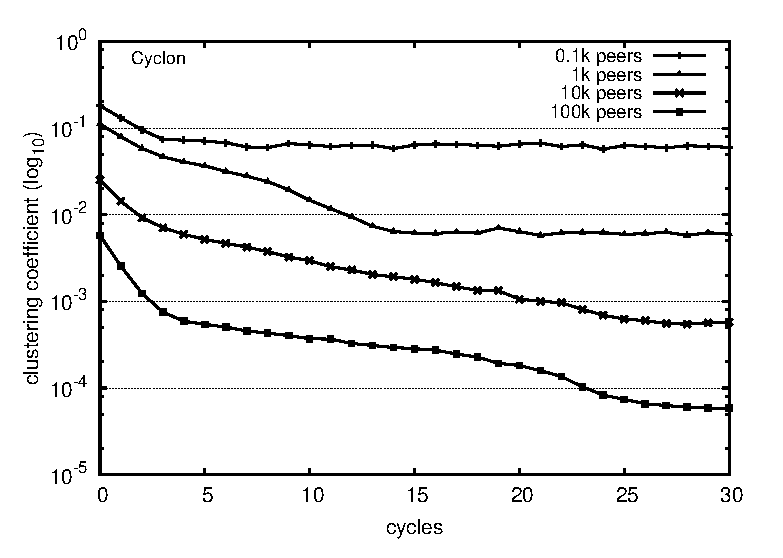
\includegraphics[width=0.47\textwidth]{img/spray/cycloncluster.eps}}
  \hspace{10pt}
  \subfloat[Figure B][Clustering coefficient of \SPRAY.]{
    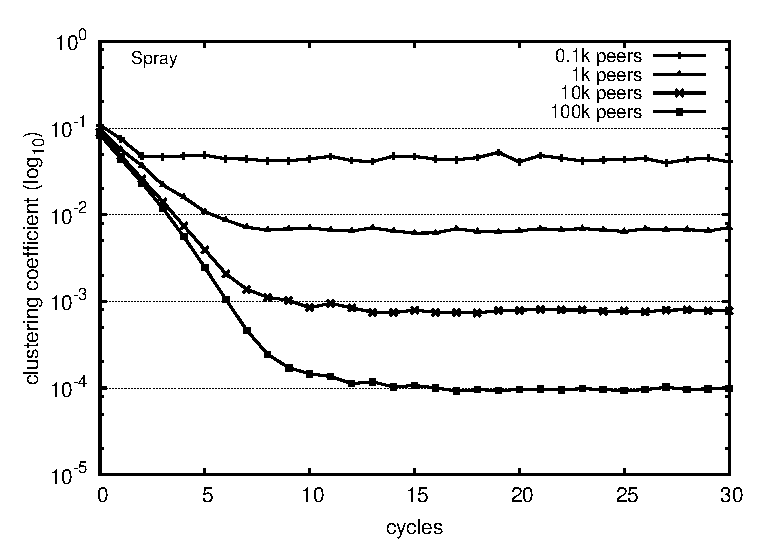
\includegraphics[width=0.47\textwidth]{img/spray/spraycluster.eps}}
  \caption{\label{fig:clustering}The x-axis denotes the elapsed time in cycles
    while the y-axis denotes the $\log_{10}$-scaled clustering coefficient.}
\end{figure*}

\begin{figure}
  \centering
  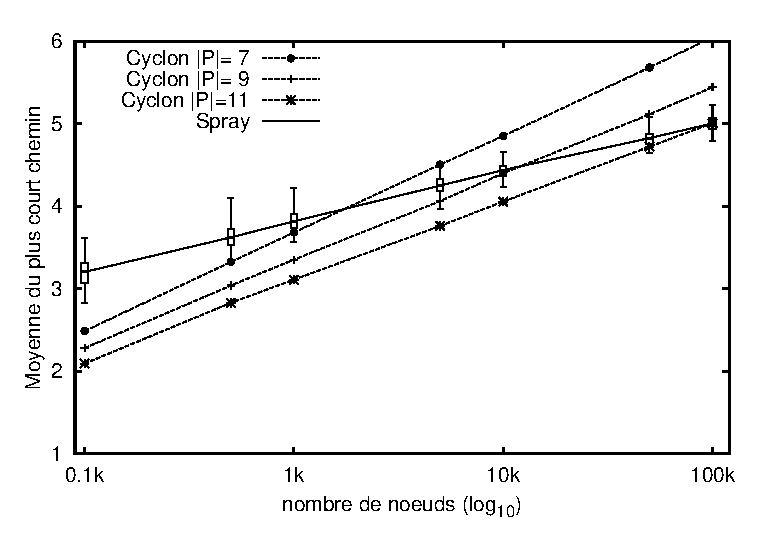
\includegraphics[width=\textwidth]{img/spray/avgpath.eps}
  \caption{\label{fig:avgpath}The average shortest path length of \SPRAY and
    \CYCLON. The x-axis denotes the number of peers in the network on a
    $\log_{10}$ scale (from 100 to 100k peers) while the y-axis denotes the
    average shortest path length of the network.}
\end{figure}

\begin{figure}
  \centering
  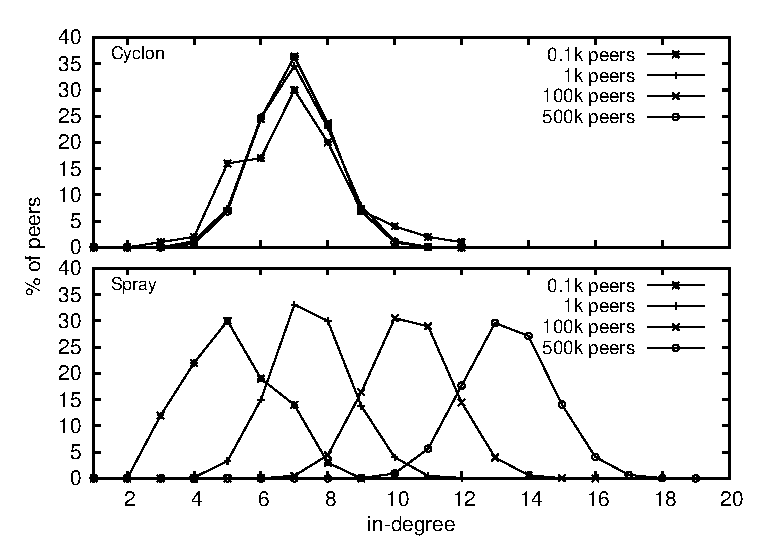
\includegraphics[width=\textwidth]{img/spray/histo.eps}
  \caption{\label{fig:histo}The in-degree distribution of \CYCLON and
    \SPRAY. The x-axis denotes the in-degree in number of nodes while the
    y-axis indicates the percentage of peers with such in-degree. The top
    figure is dedicated to the runs concerning \CYCLON while the bottom figure
    concerns \SPRAY.}
\end{figure}

\begin{figure*}
  \centering
  \subfloat[Figure A][\label{fig:churnA}The x-axis denotes the
  elapsed time in cycles. The upper graph y-axis shows the number of total
  connections in the overlay while the lower graph y-axis shows the variance
  $\sigma^2$ of the partial view sizes in the network.]{
    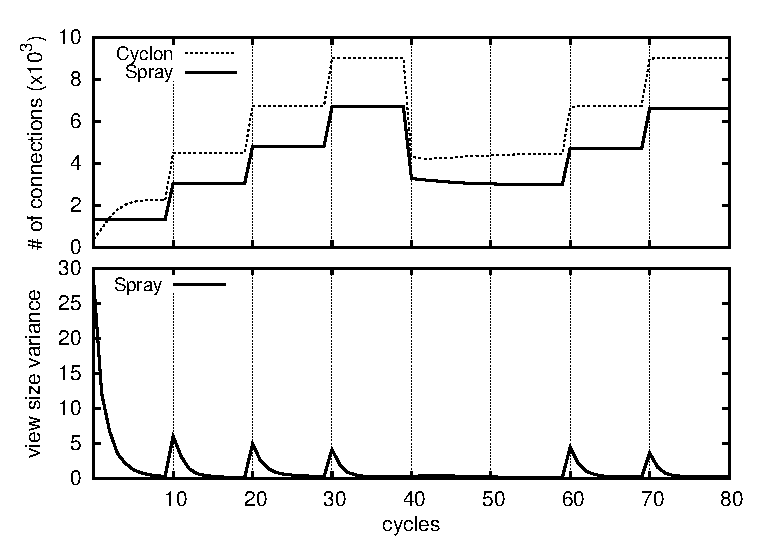
\includegraphics[width=0.47\textwidth]{img/spray/churn.eps}}
  \hspace{10pt}
  \subfloat[Figure B][\label{fig:churnB}The x-axis denotes the
  elapsed time in cycles. The y-axis denotes the average partial view size.]{
    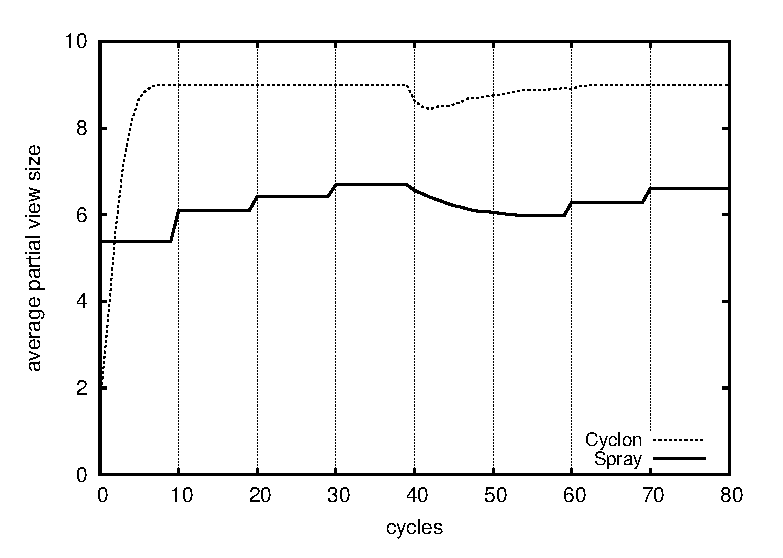
\includegraphics[width=0.47\textwidth]{img/spray/avgpv.eps}}
  \caption{\label{fig:churn}\CYCLON (partial view size configured to 9) and
    \SPRAY in a dynamic network. 2.5k peers join the network at cycles $0$,
    $10$, $20$, and $30$. Then 5k peers leave at cycle $40$. Finally 2.5k peers
    join at cycles $60$ and $70$. The final network contains 10k members.}
\end{figure*}

\begin{figure}
  \centering
  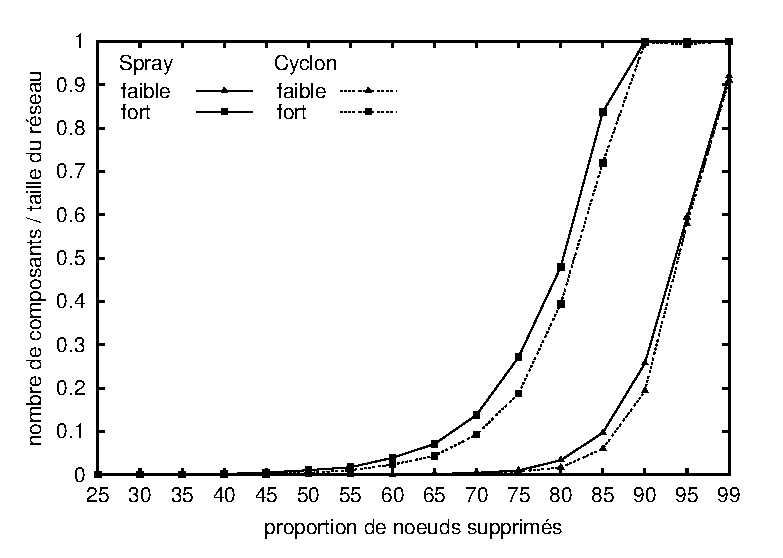
\includegraphics[width=\textwidth]{img/spray/resilience.eps}
  \caption{\label{fig:resilience}Robustness of \CYCLON and \SPRAY to massive
    failures. The x-axis denotes the percentage of peers removed at once in a
    network containing 10k members. The y-axis denotes the number of
    components over the current network size (after the removals). The
    measurements concern the weak and strong components which basically means
    the number clusters in undirected or directed graph respectively.}
\end{figure}


\begin{figure}
  \centering
  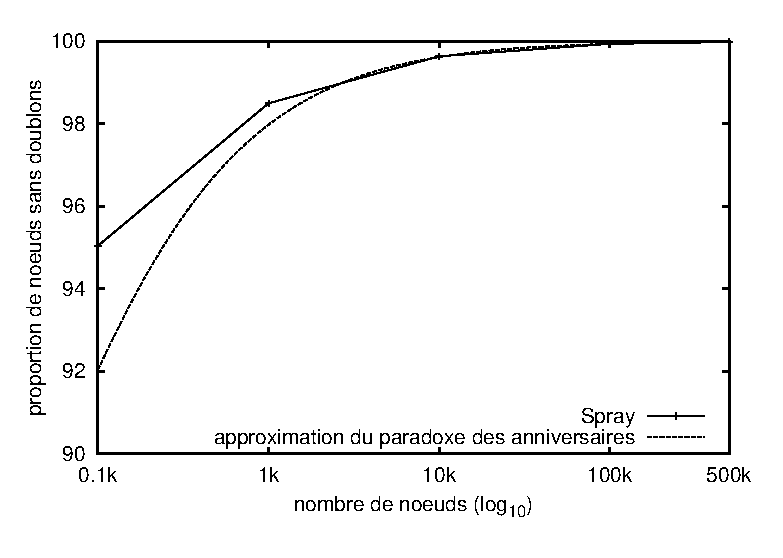
\includegraphics[width=\textwidth]{img/spray/duplicates.eps}
  \caption{\label{fig:duplicates}Duplicates in networks of different size: the
    $\log_{10}$-scaled x-axis denotes the network size while y-axis denotes the
    proportion of peers without any duplicates in their partial view.}
\end{figure}

\begin{figure}
  \centering 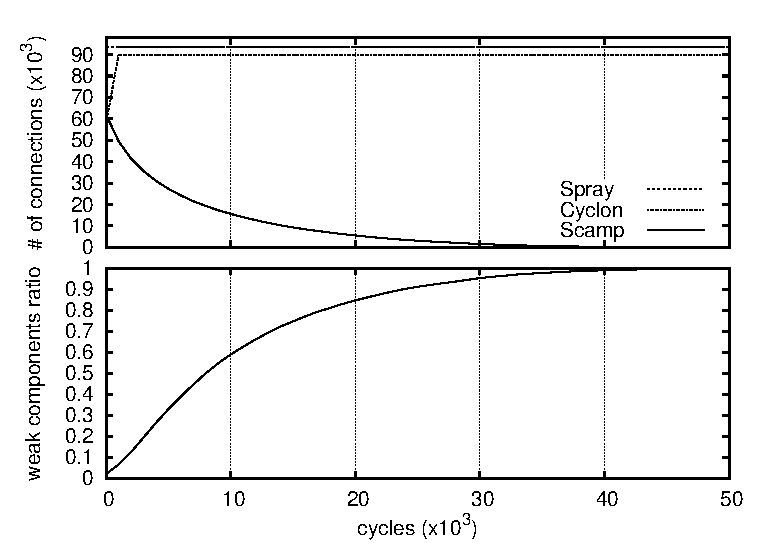
\includegraphics[width=\textwidth]{img/spray/degen.eps}
  \caption{\label{fig:degeneration}\CYCLON, \SCAMP, and \SPRAY in network
    subject to failures in the connection establishments. The x-axis denotes
    the elapsed time in cycles ($10^3$-scaled). The y-axis of the top figure
    denotes the global number of arcs ($10^3$-scaled). The y-axis of the bottom
    figure denotes the ratio of weak components over the current network size.}
\end{figure}

%%% Local Variables:
%%% mode: latex
%%% TeX-master: "../../paper"
%%% End:


\section{Conclusion}


%%% Local Variables:
%%% mode: latex
%%% TeX-master: "../../paper"
%%% End:

% 
\chapter{Éditeur collaboratif réparti}


\section{Introduction}

%%% Local Variables:
%%% mode: latex
%%% TeX-master: "../../paper"
%%% End:


\section{CRATE}

%%% Local Variables:
%%% mode: latex
%%% TeX-master: "../../paper"
%%% End:


\section{Expérimentations}


%%% Local Variables:
%%% mode: latex
%%% TeX-master: "../../paper"
%%% End:


\section{Conclusion}

%%% Local Variables:
%%% mode: latex
%%% TeX-master: "../../paper"
%%% End:



%%% Local Variables:
%%% mode: latex
%%% TeX-master: "../../paper"
%%% End:

% 

\chapter{Conclusion}

\minitoc


\section{Conclusion}

%%% Local Variables:
%%% mode: latex
%%% TeX-master: "../../paper"
%%% End:


\section{Perspectives}
\label{conclu:sec:perspectives}

%Les travaux réalisés lors de cette thèse et présenté dans ce manuscrit offrent
%de nombreuses perspectives de différente granularité. 
Tout d'abord, chacun des composants de notre éditeur collaboratif peut être
amélioré ou étendu. Ensuite, l'éditeur lui-même offre des opportunités
inédites. Par exemple, son intégration, non en opposition, mais en complément
des approches actuellement centralisés. Enfin, l'architecture ouvre aussi la
voie à un plus large champs d'applications décentralisées directement
accessibles via les navigateurs Web.

Cette section fournit une liste de perspectives scientifiques concernant ces
travaux de thèse.

\subsection{Fusion de réseaux}

\label{conclu:subsec:merging}

La fusion de réseaux consiste à obtenir un réseau unique comme l'union des
membres de plusieurs réseaux. Le réseau obtenu doit hériter des propriétés de
ses parents.  Lors de ce processus, nous supposons qu'au moins un des nœuds
appartenant à l'un des réseau contacte l'autre réseau afin d'initier la
fusion. Grâce à la connexion qui en résulte, les réseaux sont à même de
communiquer, et donc de fusionner.

Les approches à taille fixe sont triviales à étendre : les mélanges périodiques
suffisent à garantir un réseau connexe. Si toutefois les vues partielles sont
configurées avec des tailles différentes, il suffit alors de prendre la taille
maximum des deux. Par exemple, un nœud avec une vue partielle de 5 voisins verra
sa vue augmenter à $7$ voisins après un échange avec le nœud dont la vue
partielle est peuplée de $7$ références.

\SPRAY est une approche dont les vues partielles évoluent automatiquement en
réaction aux entrées et sorties du réseau. En particulier, les vues partielles
suivent une progression logarithmiques comparée à la taille du réseau. La fusion
de réseaux \SPRAY doit résulter en un réseau \SPRAY garantissant de même.

La première solution qui vient à l'esprit est la suivante : chacun des nœuds du
premier réseau utilise le contact afin de rejoindre le second réseau, comme un
sablier dont les grains passent un tube étroit pour rejoindre l'autre bulbe sous
l'effet de la gravité. Malheureusement, cette solution est extrêmement lente --
puisque la majorité des nœuds ignorent encore qui est le contact -- et
susceptible d'échouer -- puisque le contact est un point unique de défaillance.

Un seconde solution consiste simplement, à l'instar des approches à taille fixe,
à laisser le mécanisme de mélange faire son office. Petit à petit, d'autres
ponts entre les réseaux vont se former jusqu'à ce que les deux réseaux soient
indifférenciés. Malheureusement, les arcs ne suivent pas l'augmentation relative
au réseau.

\begin{problem}
  Soit $\mathcal{N}_1,\, \mathcal{N}_2,\, \ldots ,\, \mathcal{N}_k$ des réseaux
  de taille arbitraire. On a :
\begin{equation}
  \sum\limits_{i \in \mathbb{N}_{<k}} |\mathcal{N}_i|\ln (|\mathcal{N}_i|) < (\sum\limits_{i \in \mathbb{N}_{<k}} |\mathcal{N}_i|)\ln{(\sum\limits_{i \in \mathbb{N}_{<k}} |\mathcal{N}_i|)}
\end{equation}
Comment adapter les nombres d'arcs effectif (à gauche) pour qu'il atteigne le
nombre d'arcs requis (à droite)?
\end{problem}


% Pour répondre à ce problème, chacun des nœuds appartenant aux réseaux impliqués
% dans la fusion doit être capable de
% \begin{inparaenum}[(i)]
% \item détecter lorsqu'un nouveau réseau fusionne avec celui dans lequel il se
%   trouve (cf. §\ref{net:subsec:detection}),
% \item détecter lorsqu'il a glané suffisamment d'informations pour procéder à la
%   fusion (cf. §\ref{net:subsec:activation}),
% \item ajuster sa vue partielle en conséquence (cf. §\ref{net:subsec:merging}).
% \end{inparaenum}

\subsection{Table de hachage répartie}

Une table de hachage répartie (\emph{DHT}\footnote{\emph{Distributed Hash
    Table}}) est un système permettant de retrouver une ressource rapidement
dans un réseau superposé de nœuds. La ressource recherchée possède une clé
permettant l'exploration efficace du réseau.

Parmi les représentants des DHT on trouve Chord~\cite{stoica2001chord},
CAN~\cite{ratnasamy2001scalable}, Pastry~\cite{rowstron2001pastry},
Tapestry~\cite{zhao2006tapestry}, Kademlia~\cite{maymounkov2002kademlia}, ou
Kelips~\cite{gupta2003kelips}.  Ces approches font souvent état d'une vue
partielle logarithmique.  Toutefois, tout comme pour les protocoles
d'échantillonnage aléatoire de pairs dont la vue partielle est fixe, tel que
\CYCLON, la taille de leur vue est configurée par avance. Lorsque le système
fait face à de fréquentes entrées et sorties de nœuds, les vues peuvent être
ajustées grâce à des mécanismes d'estimation de la taille du
réseau~\cite{camarillo2014self, ghinita2006adaptive}. Cependant, ces mécanismes
présentent un coût additionnel~\cite{ghinita2006adaptive}.

\begin{figure}
  \begin{center}
    
\begin{tikzpicture}[scale=1.2]

  \newcommand\X{75pt};
  \newcommand\Y{75pt};

  \newcommand\1{0.865};
  \newcommand\2{0.705};
  \newcommand\3{0.5};

  \scriptsize
  \draw[fill=white, very thick, draw=darkblue]
  (1*\X, 0*\Y) node{\DARKBLUE{$n_1$}} +(-5pt,-5pt) rectangle +(5pt,5pt);
  \draw[fill=white]
  (\1*\X, \3*\Y) node{$n_2$} +(-5pt,-5pt) rectangle +(5pt,5pt);
  \draw[fill=white]
  (\2*\X, \2*\Y) node{$n_3$} +(-5pt,-5pt) rectangle +(5pt,5pt);
  \draw[fill=white]
  (\3*\X, \1*\Y) node{$n_4$} +(-5pt,-5pt) rectangle +(5pt,5pt);
  \draw[fill=white]
  (0*\X, 1*\Y) node{$n_5$} +(-5pt,-5pt) rectangle +(5pt,5pt);
  
  \draw[->, very thick, color = darkblue](1*\X, 5+0*\Y) --
  node[anchor=west]{\DARKBLUE{\textbf{plus proche}}} (\1*\X, -5+\3*\Y);
  \draw[->](-5+\1*\X, 5+\3*\Y) -- (5+\2*\X, -5+\2*\Y);
  \draw[->](-5+\2*\X, 5+\2*\Y) -- (5+\3*\X, -5+\1*\Y);
  \draw[->](-5+\3*\X, \1*\Y) -- (5+0*\X, 1*\Y);


  \draw[fill=white]
  (-\3*\X, \1*\Y) node{$n_6$} +(-5pt,-5pt) rectangle +(5pt,5pt);
  \draw[fill=white]
  (-\2*\X, \2*\Y) node{$n_7$} +(-5pt,-5pt) rectangle +(5pt,5pt);
  \draw[fill=white]
  (-\1*\X, \3*\Y) node{$n_8$} +(-5pt,-5pt) rectangle +(5pt,5pt);
  \draw[fill=white]
  (-1*\X, 0*\Y) node{$n_9$} +(-5pt,-5pt) rectangle +(5pt,5pt);

  \draw[->](-5+0*\X, 1*\Y) -- (5+-\3*\X, \1*\Y);
  \draw[->](-5-\3*\X, -5+\1*\Y) -- (5-\2*\X, 5+\2*\Y);
  \draw[->](-5-\2*\X, -5+\2*\Y) -- (5-\1*\X, 5+\3*\Y);
  \draw[->](-\1*\X, -5+\3*\Y) -- (-1*\X, 5+0*\Y);

  \draw[fill=white]
  (-\1*\X, -\3*\Y) node{$n_{10}$} +(-5pt,-5pt) rectangle +(5pt,5pt);
  \draw[fill=white]
  (-\2*\X, -\2*\Y) node{$n_{11}$} +(-5pt,-5pt) rectangle +(5pt,5pt);
  \draw[fill=white]
  (-\3*\X, -\1*\Y) node{$n_{12}$} +(-5pt,-5pt) rectangle +(5pt,5pt);
  \draw[fill=white]
  (0*\X, -1*\Y) node{$n_{13}$} +(-5pt,-5pt) rectangle +(5pt,5pt);

  \draw[->](-1*\X, -5+0*\Y) -- (-\1*\X, 5-\3*\Y);
  \draw[->](5-\1*\X, -5-\3*\Y) -- (-5-\2*\X, 5-\2*\Y);
  \draw[->](5-\2*\X, -5-\2*\Y) -- (-5-\3*\X, 5-\1*\Y);
  \draw[->](5-\3*\X, -\1*\Y) -- (-5+0*\X, -1*\Y);

  \draw[fill=white]
  (\3*\X, -\1*\Y) node{$n_{14}$} +(-5pt,-5pt) rectangle +(5pt,5pt);
  \draw[fill=white]
  (\2*\X, -\2*\Y) node{$n_{15}$} +(-5pt,-5pt) rectangle +(5pt,5pt);
  \draw[fill=white]
  (\1*\X, -\3*\Y) node{$n_{16}$} +(-5pt,-5pt) rectangle +(5pt,5pt);

  \draw[->](5+0*\X, -1*\Y) -- (-5+\3*\X, -5-\1*\Y);
  \draw[->](5+\3*\X, -\1*\Y) -- (-5+\2*\X, -5-\2*\Y);
  \draw[->](5+\2*\X, 5-\2*\Y) -- (-5+\1*\X, -5-\3*\Y);
  \draw[->](\1*\X, 5-\3*\Y) -- (1*\X, -5+0*\Y);


  \draw[<->](0*\X, -5+1*\Y) -- (0*\X, 5+-1*\Y);
  \draw[<->](-5+\1*\X, -5+\3*\Y) -- (5-\1*\X, 5-\3*\Y);
  \draw[<->](-5+\2*\X, -5+\2*\Y) -- (5-\2*\X, 5-\2*\Y);
  \draw[<->](-5+\3*\X, -5+\1*\Y) -- (5-\3*\X, 5-\1*\Y);
  \draw[<->](-5+\1*\X, 5-\3*\Y) -- (5-\1*\X, -5+\3*\Y);
  \draw[<->](-5+\2*\X, 5-\2*\Y) -- (5-\2*\X, -5+\2*\Y);
  \draw[<->](-5+\3*\X, 5-\1*\Y) -- (5-\3*\X, -5+\1*\Y);


  \draw[->] (-5+\1*\X, \3*\Y) -- (5-\2*\X , \2*\Y); %% 2-> 7
  \draw[->] (-5+\2*\X, \2*\Y) -- (5-\1*\X, \3*\Y); %% 3 -> 8
%  \draw[->] (-5+\3*\X, -5+\1*\Y) -- (5-1*\X, 5+0*\Y); %% 4 -> 9
%  \draw[->] (-5+0*\X, -5+1*\Y) -- (5-\1*\X, 5-\3*\Y); %% 5 -> 10
  \draw[->] (-\3*\X, -5+\1*\Y) -- (-\2*\X, 5-\2*\Y); %% 6 -> 11
  \draw[->] (-\2*\X, -5+\2*\Y) -- (-\3*\X, 5-\1*\Y); %% 7 -> 12
  \draw[->] (5+-\1*\X, -5+\3*\Y) -- (-5+0*\X, 5-1*\Y); %% 8 -> 13
  \draw[->] (5+-1*\X, -5+0*\Y) -- (-5+\3*\X, 5-\1*\Y); %% 9 -> 14
  \draw[->] (5-\1*\X, -\3*\Y) -- (-5+\2*\X, -\2*\Y); %% 10 -> 15
%  \draw[->] (5-\2*\X, -\2*\Y) -- (-5+\1*\X, -\3*\Y); %% 11 -> 16
  \draw[->] (5-\3*\X, 5-\1*\Y) -- (-5+1*\X, -5+0*\Y); %% 12 -> 1
%  \draw[->] (5-0*\X, 5-1*\Y) -- (-5+\1*\X, -5+\3*\Y); %% 13 -> 2
  \draw[->] (\3*\X, 5-\1*\Y) -- (\2*\X, -5+\2*\Y); %% 14 -> 3
  \draw[->] (\2*\X, 5-\2*\Y) -- (\3*\X, -5+\1*\Y); %% 15 -> 4
  \draw[->] (-5+\1*\X, 5-\3*\Y) -- (5+0*\X, -5+1*\Y); %% 16 -> 5


  \draw[<->, very thick, color = darkblue](5-\X, 0*\Y) --
  node[anchor=south west]{\DARKBLUE{\textbf{\ \ \ \ plus lointain}}}(-5+\X, 0*\Y);
  \draw[->, very thick, color = darkblue] (-5+\X, 5+0*\Y) --
  node[anchor=south]{\DARKBLUE{$\mathbf{1\over{3}}$}}(5-\3*\X, -5+\1*\Y); %% 1 -> 6
\end{tikzpicture}


%%% Local Variables:
%%% mode: latex
%%% TeX-master: "../../paper"
%%% End:

    \caption[Table de hachage répartie]
    {\label{conclu:fig:dhtexample}Table de hachage répartie suivant le principe
      de Chord.}
  \end{center}
\end{figure}

Construire une DHT au dessus d'un protocole d'échantillonnage aléatoire de pairs
apporte le double avantage d'une convergence rapide vers une topologie optimale,
et d'une résilience aux fréquentes entrées et sorties de
nœuds~\cite{krasikova2016distributed, montresor2005chord,
  voulgaris2013vicinity}.  Comme le montre la
figure~\ref{conclu:fig:dhtexample}, l'idée est de placer les systèmes classiques
de DHT -- ici Chord -- afin qu'ils s'accordent avec la vue partielle fournie par
\SPRAY. Par exemple, si un nœud \SPRAY possède 3 voisins, le réseau superposé en
charge de la DHT possède lui aussi 3 voisins. Toutefois, ces derniers sont
choisis selon la distance à laquelle ils se trouvent. Un premier voisin serait
celui qui est le plus proche, le second voisin celui qui se trouve à la moitié
de la distance maximum, et le troisième se trouverait à un tiers de la distance
maximum. Un tel système permet de diriger les messages ciblant un nœud
particulier très efficacement : de l'ordre de $\log |\mathcal{N}|$ sauts en
moyenne, où $\mathcal{N}$ est l'ensemble des membres appartenant au réseau.

% \subsection{Sécurité}

% Les protocoles d'appartenance à un réseau font face à des problèmes de sécurités
% inhérents aux protocoles ciblant de larges dimensions. 

\subsection{Compromis causalité et concurrence}

\CRATE comprend une couche dédiée à la détection de relations causales. La
structure utilisée est celle d'un vecteur d'horloges incluant des
exceptions~\cite{malkhi2007concise}. Celle-ci, identiquement aux vecteurs
d'horloges, stockent localement au moins un entier par collaborateur ayant
jamais participé dans l'édition. Pour les dispositifs informatiques aux
configurations plus modestes comme les téléphones portables, la progression
linéaire de ces vecteurs constitue un problème.

Une perspective possible serait de remplacer ce vecteur d'horloges de taille
$W$, où $W$ est le nombre de membres ayant jamais participé à la session
d'édition, par un vecteur d'horloges de taille $K$, où $K$ est un entier
nettement inférieur à $W$. L'intuition derrière cette structure provient du fait
que lorsqu'il n'y a pas de concurrence, une seule horloge de
Lamport~\cite{lamport1978time} suffit pour caractériser les relations
causales. Si la concurrence augmente, alors des doublons peuvent
apparaître. L'intégration, en présence de doublons, peut conduire à des
incohérences.

L'idée serait alors d'allier
\begin{inparaenum}[(i)]
\item une structure utilisant un vecteur dont la taille s'ajuste à la
  concurrence du système afin de borner la fréquence des erreurs;
\item un mécanisme de recouvrement sur erreur afin d'intégrer l'opération
  arrivée en retard;
\item un mécanisme d'anti-entropie afin que le système soit fiable : toutes les
  opérations parviennent à tous les participants.
\end{inparaenum}

% \subsection{Wiki réparti temps réel}

% Les wikis sont des espaces de collaborations permettant à plusieurs participants
% d'éditer des pages à tour de rôle, i.e., l'édition n'est pas effectuée en temps
% réel. Le succès de l'encyclopédie \emph{Wikipédia}~\cite{wikipedia} n'est plus à
% démontrer~\cite{giles2005internet}. Cependant, le modèle même d'édition provoque
% l'apparition de conflits. Ces conflits ne concernent pas seulement des points de
% vue divergents, mais aussi des éditions placées aux même endroit dans le
% document au même moment. Les conflits doivent être résolus manuellement ce qui
% constitue une tâche complexe à tel point que les discussions quant à
% l'organisation de la rédaction ont énormément augmenté au cours du
% temps~\cite{kittur2007he}.

% Autoriser l'édition temps réel des pages de \emph{Wikipédia} permettrait à
% différent utilisateurs de voir les modifications effectués par d'autres
% collaborateurs afin d'agir en conséquence. Dans ce cas, les seuls conflits
% restants seraient ceux d'ordre sémantique.  De plus, décentraliser ces sessions
% d'édition temps réel permettrait de soulager le fournisseur du service des coûts
% liés à l'édition. Les membres d'une session d'édition participeraient seuls au
% bon fonctionnement de la session. Une fois le travail accompli, le document est
% sauvegardé sur le serveur et versionné normalement. Seul la sauvegarde finale
% reste de sa responsabilité.

% Enfin, \CRATE permet de placer des liens à d'autres sessions d'édition dans le
% document. Ce simple mécanisme permet de naviguer d'un document à l'autre, d'une
% session d'édition à l'autre, et plus généralement d'un réseau à un autre. Il est
% alors possible de naviguer très simplement parmi ces réseaux, pour peu qu'ils
% soient encore vivants et accessibles.

% Certains projets, comme \emph{The Fold}
% bénéficient d'une foule de gens volontaires qui mettent leur machine à
% disposition afin d'améliorer la puissance calculatoire du système.

\subsection{O'Browser, Where Art Thou?}

De nos jours, les navigateurs Web sont plus que de simples visualisateurs de
contenu, ils sont presque devenus des systèmes d'exploitation. Ils comptent
parmi les programmes les plus distribués de par le monde. Ils apparaissent dans
un large éventail d'appareils aux diverses capacités tels que les mobiles, les
tablettes, ou les ordinateurs de bureaux.

Développer une application Web, c'est développer pour une large audience
hétérogène.  L'éditeur collaboratif temps réel \CRATE prouve qu'il est possible
de développer des applications décentralisées directement dans le navigateur
Web. Le projet WebTorrent~\cite{webtorrent} constitue un autre exemple
d'application décentralisée fonctionnant dans le navigateur Web. Ce projet
permet le transfert de fichiers statique. Quelles autres applications
décentralisées est-il possible de développer ?

Rassembler l'ensemble des composants répartis en un langage adapté au Web
permettrait de développer un catalogue d'applications décentralisées
garantissant certaines propriétés sur, par exemple, le critère de cohérence ou
la sécurité. \CRATE ne serait que l'une des applications temps réel que ce
langage permettrait d'écrire. Cela constituerait une avancée certaine en faveur
d'un Web décentralisé. De surcroît, lorsque des navigateurs Web sont
actuellement entièrement développés dans l'optique de supporter le
décentralisé~\cite{maelstrom} -- ce qui représente une dépense substantielle --
le même objectif pourrait être atteint en étendant simplement les capacités des
navigateurs Web existants.


%%% Local Variables:
%%% mode: latex
%%% TeX-master: "../../paper"
%%% End:


%%% Local Variables:
%%% mode: latex
%%% TeX-master: "../../paper"
%%% End:


\bibliographystyle{plain}
\bibliography{bibliographie}

%\backmatter
\end{document}

%%% Local Variables:
%%% mode: latex
%%% ispell-local-dictionary: "fr"
%%% eval: (flyspell-mode 1)
%%% End: